\chapter{Theoretical Background}
\label{cha:theory}

\section{Statistical Thermodynamics and Free Energy}
\label{sec:freeE}

In the following, a brief introduction to the broad field of free energy calculation\autocite{chipot2007free} and more specific to the idea of \textit{enhanced sampling}\autocite{bernardi2015enhanced,abrams2014enhanced} is given.
Considering a system of atoms with coordinates $\textbf{x}^T=(x_1,...,x_{3N})$ and momenta $\textbf{p}^T=(p_1,...,p_{3N})$, the total energy is given by the Hamiltonian
\begin{equation}
  H(\textbf{x},\textbf{p})=\sum_{i=1}^{3N}\frac{p_{i}^{ 2}}{2 M_i} + U(\textbf{x}),
  \label{eq:lagrangian}
\end{equation}
where $M$ denotes the mass of atomic nuclei, which are treated classically, and $U(\textbf{x})$ is the Born-Oppenheimer potential energy surface (PES).\autocite{combes1981born}
In practice the PES can ether be obtained from molecular mechanics (MM) using some force field\autocite{ponder2003force} or from a quantum mechanical electronic structure theory (QM), most commonly density functional theory (DFT).\autocite{burke2012perspective}
If the system is in thermal equilibrium the probability density $\rho(\textbf{x})$ in configuration space $\textbf{x}$ at temperature $T$ is given by the Boltzmann distribution
\begin{equation}
  \rho(\textbf{x})=\frac{e^{-\beta U(\textbf{x})}}{\int e^{-\beta U(\textbf{x})} d\textbf{x}}=Z^{-1}e^{-\beta U(\textbf{x})}
  \label{eq:boltzmann}
\end{equation}
$Z$ denotes the \textit{configuration integral} and $\beta=(k_B T)^{-1}$ with the Boltzmann constant $k_B$.\autocite{chipot2007free}
In this thesis the focus is on chemical reactions, $A \longrightarrow B$, which are represented by collective variables (CVs)
\begin{equation}
 \xi(\textbf{x}) : \mathbb{R} ^{3N} \to \mathbb{R}
\end{equation}
that are sufficient to distinguish between key states of interest.
Typical CVs are for example atomic distances, bend angles, or dihedrals (details are given in the Appendix).\autocite{fiorin2013using}
%Because of the rapid growing computational effort for sampling of multidimensional coordinates we will only consider 1 or 2 dimensional CVs in the following.
The marginal probability distribution of these CVs is defined by
\begin{equation}
  \rho(z)=\int \delta[\xi(\textbf{x})-z]\rho(\textbf{x})d\textbf{x}=\braket{\delta [\xi(\textbf{x})-z]}_z
  \label{eq:rho}
\end{equation}
where $\braket{}_z$ denotes the $z$-conditioned marginal distribution.\autocite{chipot2007free}
In practice the low (in the following maximal two) dimensional probability density $\rho(z)$ is expressed by a histogram with fixed bin size $\delta z$.
The potential of mean force (PMF) $A(z)$, i.e., potential of the canonical (N,V,T)-ensemble, is defined as
\begin{equation}
  A(z) = -\beta^{-1}\ln \rho(z)
  \label{eq:free energy}
\end{equation}
Note that the shape of the PMF is not gauge invariant against the choice of CV function $\xi$.
Therefore features of the PMF like minima or transition barriers have no CV independent meaning.\autocite{hartmann2011two}
This is, however, not problematic for the calculation of free energy differences, because the CV dependent feature is integrated out to obtain the probability if the system occupies state A or B.
\begin{equation}
  \Delta A_{A\rightarrow B} = -\beta^{-1}\ln \frac{\int_B \rho(z)dz}{\int_A \rho(z)dz}=-\beta^{-1}\ln \frac{p_B}{p_A}
  \label{eq:free energy diff}
\end{equation}
However, it is impossible to directly calculate the direct configuration-space integrals used in equation \ref{eq:boltzmann} and \ref{eq:rho}.\autocite{chipot2007free}
Most developments in the area of free energy estimation therefore rely on the concept of \textit{ergodicity}\autocite{schutte2013metastability}, which states that each point in phase space converges to a unique limiting value for $t\rightarrow\infty$, such that the time average is equal to the ensemble average\autocite{barducci2011metadynamics}

\begin{equation}
   \lim_{t\to\infty}\frac{1}{t} \int_0^t \rho(z(t')) dt' = \braket{\delta [\xi(\textbf{x})-z]}_z
  \label{eq:ergodic}
\end{equation}
This allows for the calculation of statistically averaged properties from simulations of trajectories, which can for example be obtained from molecular dynamics (MD) or Monte Carlo (MC) simulations.
However, the PMF of chemical reactions is often characterized by many metastable states, which are separated by free energy barriers much larger then the thermal energy $k_B T$.
Therefore, on timescales we can simulate, MD or MC trajectories stay kinetically trapped and are unable to explore the full reaction coordinate.
In other words most chemical processes behave \textit{quasi-nonergodic} in the computationally accessible time frame, which often renders brute-force sampling of reaction coordinates in single trajectories virtually impossible.
%The problem of calculating accurate free energy differences hence really consists in adequate sampling of regions with high free energy (transition states) along the reaction coordinate.

To circumvent this problem countless \textit{enhanced sampling} algorithms were proposed to enable efficient sampling of the hole reaction coordinate.\autocite{jiang2010free, sugita1999replica,den2000thermodynamic, kastner2011umbrella, ciccotti2005blue, barducci2008well}
In this work we will focus on CV-based approaches, that alter either the potential energy $U$ or the molecular forces $\textbf{F}$ of a system in a way, that increases the time spent in important regions of configuration space during a simulation.
One of the oldest and simplest methods to achieve the same is \textit{Umbrella Sampling} (US)\autocite{kastner2011umbrella}, which introduces fixed harmonic bias potentials to restrain the simulation to a given window in CV space and will be introduced in the following section.
The main focus of this work lies on \textit{Adaptive Biasing Methods} \autocite{barducci2011metadynamics,comer2015adaptive, lesage2017smoothed}, which aim for uniform sampling along the reaction coordinate by using a history dependent biasing term (section \ref{sec:adaptive biasing}).

\section{Umbrella Sampling (US)}
In its most common form US introduces a fixed harmonic bias potential of the form
\begin{equation}
  U_i^B(\xi) = \frac{k_i}{2}(\xi(\textbf{x})-\xi_i)^2 \label{eq:US bias}
\end{equation}
where the index i indicates a given bias window along the reaction coordinate with force constant $k_i$.\autocite{kastner2011umbrella} From simulations in window i the biased probability distribution $P_i^B(z)$ is obtained\autocite{kumar1992weighted}
\begin{equation}
\begin{split}
  P_i^B(z) &= \frac{\int d\textbf{x} e^{-\beta (U(\textbf{x})+U_i^B(\xi(\textbf{x})))}\delta[\xi(\textbf{x})-z]}
  {\int d\textbf{x} e^{-\beta (U(\textbf{x})+U_i^B(\xi(\textbf{x})))}} \\
             &= \frac{e^{-\beta U_i^B(z)}}{\int e^{-\beta (U(\textbf{x})+U_i^B(\xi(\textbf{x})))}d\textbf{x}} \int d\textbf{x} e^{-\beta U(\textbf{x})}\delta[\xi(\textbf{x})-z]
\end{split}
\end{equation}
Using equation \ref{eq:boltzmann} and \ref{eq:rho} the connection of $P_i^B$ to the unbiased probability distribution $P_i^0$ can be derived.
\begin{equation}
\begin{split}
  P_i^0(z) &= P_i^B(z)e^{\beta U_i^B(z)}\frac{\int e^{-\beta (U(\textbf{x})+U_i^B(\xi(\textbf{x})))}d\textbf{x}} {\int e^{-\beta U(\textbf{x})}d\textbf{x}} \\
  &= P_i^B(z)e^{\beta U_i^B(z)}\frac{Z_B}{Z_0}
\end{split}
\end{equation}
Inserting into equation \ref{eq:free energy} gives the unbiased PMF
\begin{equation}
  \begin{split}
  A_i(z) &= -\beta^{-1}\ln P_i^B(z) - U_i^B(z) - \beta^{-1}\ln\frac{Z_B}{Z_0} \\
           &= A_i^B(z) - U_i^B(z) - F_i \label{eq:A US}
  \end{split}
\end{equation}
The last term of equation (\ref{eq:A US}) is the free energy difference between the unbiased and biased system.
Since it is only an additive constant it does not change relative free energies computed from one window.\autocite{kumar1992weighted}
However, to enhance sampling of CV space typically multiple windows, each individually covering only a small section of the reaction coordinate, are sampled. In this case the global unbiased distribution of all combined windows can be obtained from the \textit{Weighted Histogram Analysis Method} (WHAM).\autocite{souaille2001extension} The goal of WHAM is to choose the weights $p_i(z)$ in order to minimize the statistical error of the global unbiased probability density of $S$ combined simulations
\begin{equation}
  P(z)=\sum_i^{S} p_i(z) P_i^0(z)
\end{equation}
under the constraint $\sum p_i = 1$. This is achieved by the iterative solution of the self-consistent WHAM equations
\begin{equation}
  p_i(z) = \frac{N_i \e^{-\beta_i U_i^B(z)+\beta_i F_i}}{\sum_j^S N_j \e^{-\beta_j U_j^B(z)+\beta_j F_j}} \label{eq:WHAM 1}
\end{equation}
\begin{equation}
  \e^{-\beta_i F_i} = \int P(z)\e^{-\beta_i U_i^B (z)}dz
  \label{eq:WHAM 2}
\end{equation}
where $F_i$ enters equation (\ref{eq:WHAM 1}) and $P$ enters equation (\ref{eq:WHAM 2}).\autocite{kastner2011umbrella,souaille2001extension} $N_i$ is the number of samples collected in window i.
The biggest advantage of this approach is that all windows can be simulated in parallel and only have to be combined once to solve the WHAM equations. In this way, extensive sampling of the reaction coordinate can be obtained efficiently.
However, the biasing potentials have to be chosen manually for each window, requiring some knowledge of the free energy surfaces prior to the simulation.
Additionally, the requirement of overlap between windows often adds up to 50\% of the total simulation time.\autocite{comer2015adaptive}
In the next section we will look at different approaches to eliminate both drawbacks by replacing equation \ref{eq:US bias} with time dependent terms, which evolve during the simulation to achieve uniform sampling of the reaction coordinate in a single simulation.

\newpage
\section{Adaptive Biasing Methods}
\label{sec:adaptive biasing}

Instead of dividing the reaction coordinate into several windows, with adaptive biasing methods the PMF can be estimated in one single simulation. For this purpose free energy barriers along the reaction coordinate are compensated by history-dependent biasing potentials or forces. In contrast to other importance sampling strategies like umbrella sampling, this methods require no knowledge of the PMF prior to the simulation, because the bias is not chosen manually. Instead, the biasing potential automatically adapts during the simulation to enable random walk dynamics and uniform sampling in CV space.\autocite{comer2015adaptive, barducci2011metadynamics}

There are multiple adaptive biasing methods available, only differing in the construction of the bias. Potential based methods like metadynamics (MtD) disfavor already visited states by accumulating repulsive potentials along the CV (section \ref{sec:metaD}), while adaptive biasing force (ABF) methods compensate the mean force along the reaction coordinate (section \ref{sec:ABF}). Finally, as discussed in section \ref{sec:eABF}, using an extended Lagrangian, the technical requirements of ABF can be lifted without loosing its rigorous convergence behavior.\autocite{lesage2017smoothed} Additionally, this framework enables the combination of repulsive MtD potentials with ABF (meta-eABF/WTM-eABF), to unite the benefits of both approaches.\autocite{fu2018zooming,fu2019taming}

Although not necessary, stratification can increase the convergence of all adaptive biasing methods significantly. However, in contrast to US simulations, no WHAM and hence no overlap between ascending windows is required. For example in ABF simulations the global PMF can be recovered by simply joining the force estimates of all simulations.\autocite{comer2015adaptive}
To parallelize calculations one can also think of many different multiple-walker strategies.\autocite{wilson2011molecular,comer2014calculation,minoukadeh2010potential}
\textit{Shared adaptive biasing}, which is one of the simplest schemes, will be discussed in section \ref{sec:MW}.

In principle adaptive biasing methods only rely on sampling of the canonical ensemble, which will be obtained using Langevin dynamics in this work. However, all methods can also be applied in combination with other MD or MC schemes. A schematic procedure of adaptively biased Langevin dynamics is given in Algorithm \ref{alg:ABM}.

\begin{algorithm}[H]
  \caption{Velocity Verlet integrator for adaptively biased Langevin dynamics with mass tensor $\textbf{M}$, coordinates $\textbf{x}(t)$, momenta $\textbf{p}(t)$, potential $U(\textbf{x}(t))$, forces $\textbf{F}(\textbf{x}(t))$ and friction coefficient $\gamma$,}
  \label{alg:ABM}
    \begin{algorithmic}
      \WHILE{$t < t_{end}$}
        \STATE
        \STATE $\textbf{p}(t+\frac{1}{2}\Delta t) \leftarrow \textbf{p}(t) + \frac{1}{2} \bigl(\textbf{F}(\textbf{x}(t))dt-\gamma \textbf{M}^{-1}\textbf{p}(t) dt + \sqrt{2\gamma\beta^{-1}}dW_t \bigr)$
        \STATE $\textbf{x}(t+\Delta t) \leftarrow \textbf{x}(t) + \frac{2}{2+\gamma dt}\textbf{M}^{-1} \textbf{p}(t+\frac{1}{2}\Delta t) dt$
        \STATE /* Langevin dynamics
        \STATE
        \STATE $\textbf{F}(\textbf{x}(t+\Delta t)) \leftarrow -\nabla U(\textbf{x}(t+\Delta t))$
        \STATE /* get physical QM/MM forces
        \STATE
        \STATE $\xi \leftarrow f(\textbf{x}(t+\Delta t))$
        \STATE /* Calculate reaction coordinate from Cartesian coordinates
        \STATE
        \IF{$\xi_{min}\leq\xi\leq\xi_{max}$}
          \STATE
          \STATE $F_{B}(\xi, t+\Delta t))\leftarrow F_{B}(\xi, t))+\Delta F_{B}(\xi,t+\Delta t))$
          \STATE /* update history dependent bias force along reaction coordinate incrementally
          \STATE
          \STATE $\textbf{F}(\textbf{x}(t+\Delta t)) \leftarrow -\nabla U(\textbf{x}(t+\Delta t)) + F_{B}(\xi, t+\Delta t))\nabla\xi$
          \STATE /* Add biasing force to physical force
          \STATE
        \ELSE
          \STATE
          \STATE $\textbf{F}(\textbf{x}(t+\Delta t)) \leftarrow \textbf{F}(\textbf{x}(t+\Delta t)) + k\min(|\xi-\xi_{min}|,|\xi-\xi_{max}|)\nabla\xi$
          \STATE /* confine system to range of interest with harmonic constraining force
          \STATE
        \ENDIF
        \STATE
        \STATE $\textbf{p}(t+\Delta t) \leftarrow \frac{2 - \gamma dt}{2+\gamma dt} \textbf{p}(t+\frac{1}{2}\Delta t) - \frac{1}{2} \bigl(\textbf{F}(\textbf{x}(t+\Delta t))dt-\gamma \textbf{M}^{-1}\textbf{p}(t+\frac{1}{2}\Delta t)) dt + \sqrt{2\gamma\beta^{-1}}dW\bigr)$
        \STATE /* Langevin dynamics
        \STATE
      \ENDWHILE
    \end{algorithmic}
\end{algorithm}

\newpage
\subsection{(Well-Tempered) Metadynamics (MtD/WTM)}
\label{sec:metaD}
MtD biases a systems dynamic towards undersampled regions along the reaction coordinate $\xi(\textbf{x})$, by accumulating repulsive potentials in regions that have already been visited.\autocite{barducci2011metadynamics} The bias potential is typically build by a superposition of Gaussian hills and can be written
\begin{equation}
  U^{MtD}(\xi,t)= \sum_{t'=\tau_G,2\tau_G,...}^{t'<t} W \prod_{i=1}^{N_{dim}} \exp\biggr(-\frac{1}{2\sigma_{G,i}^{2}} (\xi_{i}(\textbf{x}(t))-\xi_{i}(\textbf{x}(t')))^2 \biggl),
  \label{eq:U_mtD}
\end{equation}
with deposition rate $\tau_G$ and Gaussian height and variance $W$ and $\sigma_{G,i}^2$ as free input parameters.
In practice typically maximum 2 dimensional CVs are considered.
Over time Gaussian hills are accumulated in local minima of the CV and the system is pushed towards regions with higher free energy by the biasing force $\frac{\partial U^{MtD}(\xi,t)}{\partial\xi(\textbf{x})}\nabla\xi(\textbf{x})$.
Inserting the converged MtD potential $U^{MtD}(\xi,t\to\infty)$ into equation~\ref{eq:rho} gives the new probability density.
\begin{equation}
  \begin{split}
    P^B(z) &\propto \int e^{-\beta (U(\textbf{x})+U^{MtD}(\xi,t\to\infty)}\delta[\xi(\textbf{x})-z]d\textbf{x} \\
    &\propto e^{-\beta U^{MtD}(z,t\to\infty)} P(z),
  \end{split}
\end{equation}
As $U^{MtD}(\xi,t\to\infty)$ compensates all minima of the PMF the systems evolution will resemble a random walk in CV space and $P^B(z)$ will be flat.
However, the basic assumption of metadynamics is that the free energy, as equilibrium quantity, can be estimated from non-equilibrium dynamics in which the potential energy is changed every time a new Gaussian is added.
This does not derive from any identity for the free energy, but is purely based on the observation, that $U^{MtD}(\xi,t\to\infty)$ provides an unbiased estimate of the underlying free energy surface.\autocite{bussi2006equilibrium}
\begin{equation}
  A(\xi) = -U^{MtD}(\xi, t \to \infty) + C \label{eq:F est MtD}
\end{equation}
However, as the height $W$ of newly added Gaussian's stays constant over the course of MtD simulations, eq.~\ref{eq:F est MtD} oscillates around the true PMF with errors given by $W$ and $\sigma_G$.
The bias will also grow indefinitely, which can cause numeric instabilities in the long time limit.
Well-Tempered metadynamics (WTM)\autocite{barducci2008well} addresses this issues by adding an exponential scaling factor to ensure a decrease of the Gaussian height over time:
\begin{equation}
  U^{WTM}(\xi,t) = \exp \biggl(-\frac{U^{WTM}(\xi,t-\tau_G)}{k_B \Delta T}\biggr) U^{MtD}(\xi,t)
  \label{eq:WTM}
\end{equation}
In WTM the height of newly added Gaussians evolves proportionally to the inverse of the time spent at a point in CV space. The effective temperature $\Delta T$ controls how fast the height of newly added Gaussians decreases.
For $\Delta T \to 0$ the bias is zero and ordinary MD is recovered, whereas the limit $\Delta T \to \infty$ corresponds to normal MtD.
The overall WTM potential converges to a fraction of the PMF $-\frac{\Delta T}{T+\Delta T}A(\xi)$ that is known a priori.\autocite{barducci2008well}
To again obtain the PMF from the WTM potential it is scaled with the according correction factor:
\begin{equation}
A(\xi) = -\frac{T+\Delta T}{\Delta T}U^{WTM}(\xi, t\to \infty) \label{eq:F est WTM}
\end{equation}
Figure~\ref{fig:metaD} shows a numerical example of the effect of $U^{MtD}$ and $U^{WTM}$ on the effective free energy energy surface that is sampled over the course of a simulation.
Despite its appealing theoretical and practical simplicity MtD and WTM both suffer from a rather big set of free parameters ($W$, $\tau_G$, $\sigma_G$, and $\Delta T$). All of them have significant impact on the outcome of the simulation and have to be chosen carefully. If the bias potential builds up too fast, the system is driven far away from equilibrium and the obtained free energy estimate is wrong. Small parameters on the other hand result in bad convergence behavior and inefficient sampling.\autocite{laio2005assessing}
The next section will look into ABF, which is less dependent on free parameters and stands on a more rigorous mathematical framework.

\begin{figure}[H]
    \centering
    \subfloat[Metadynamics]{{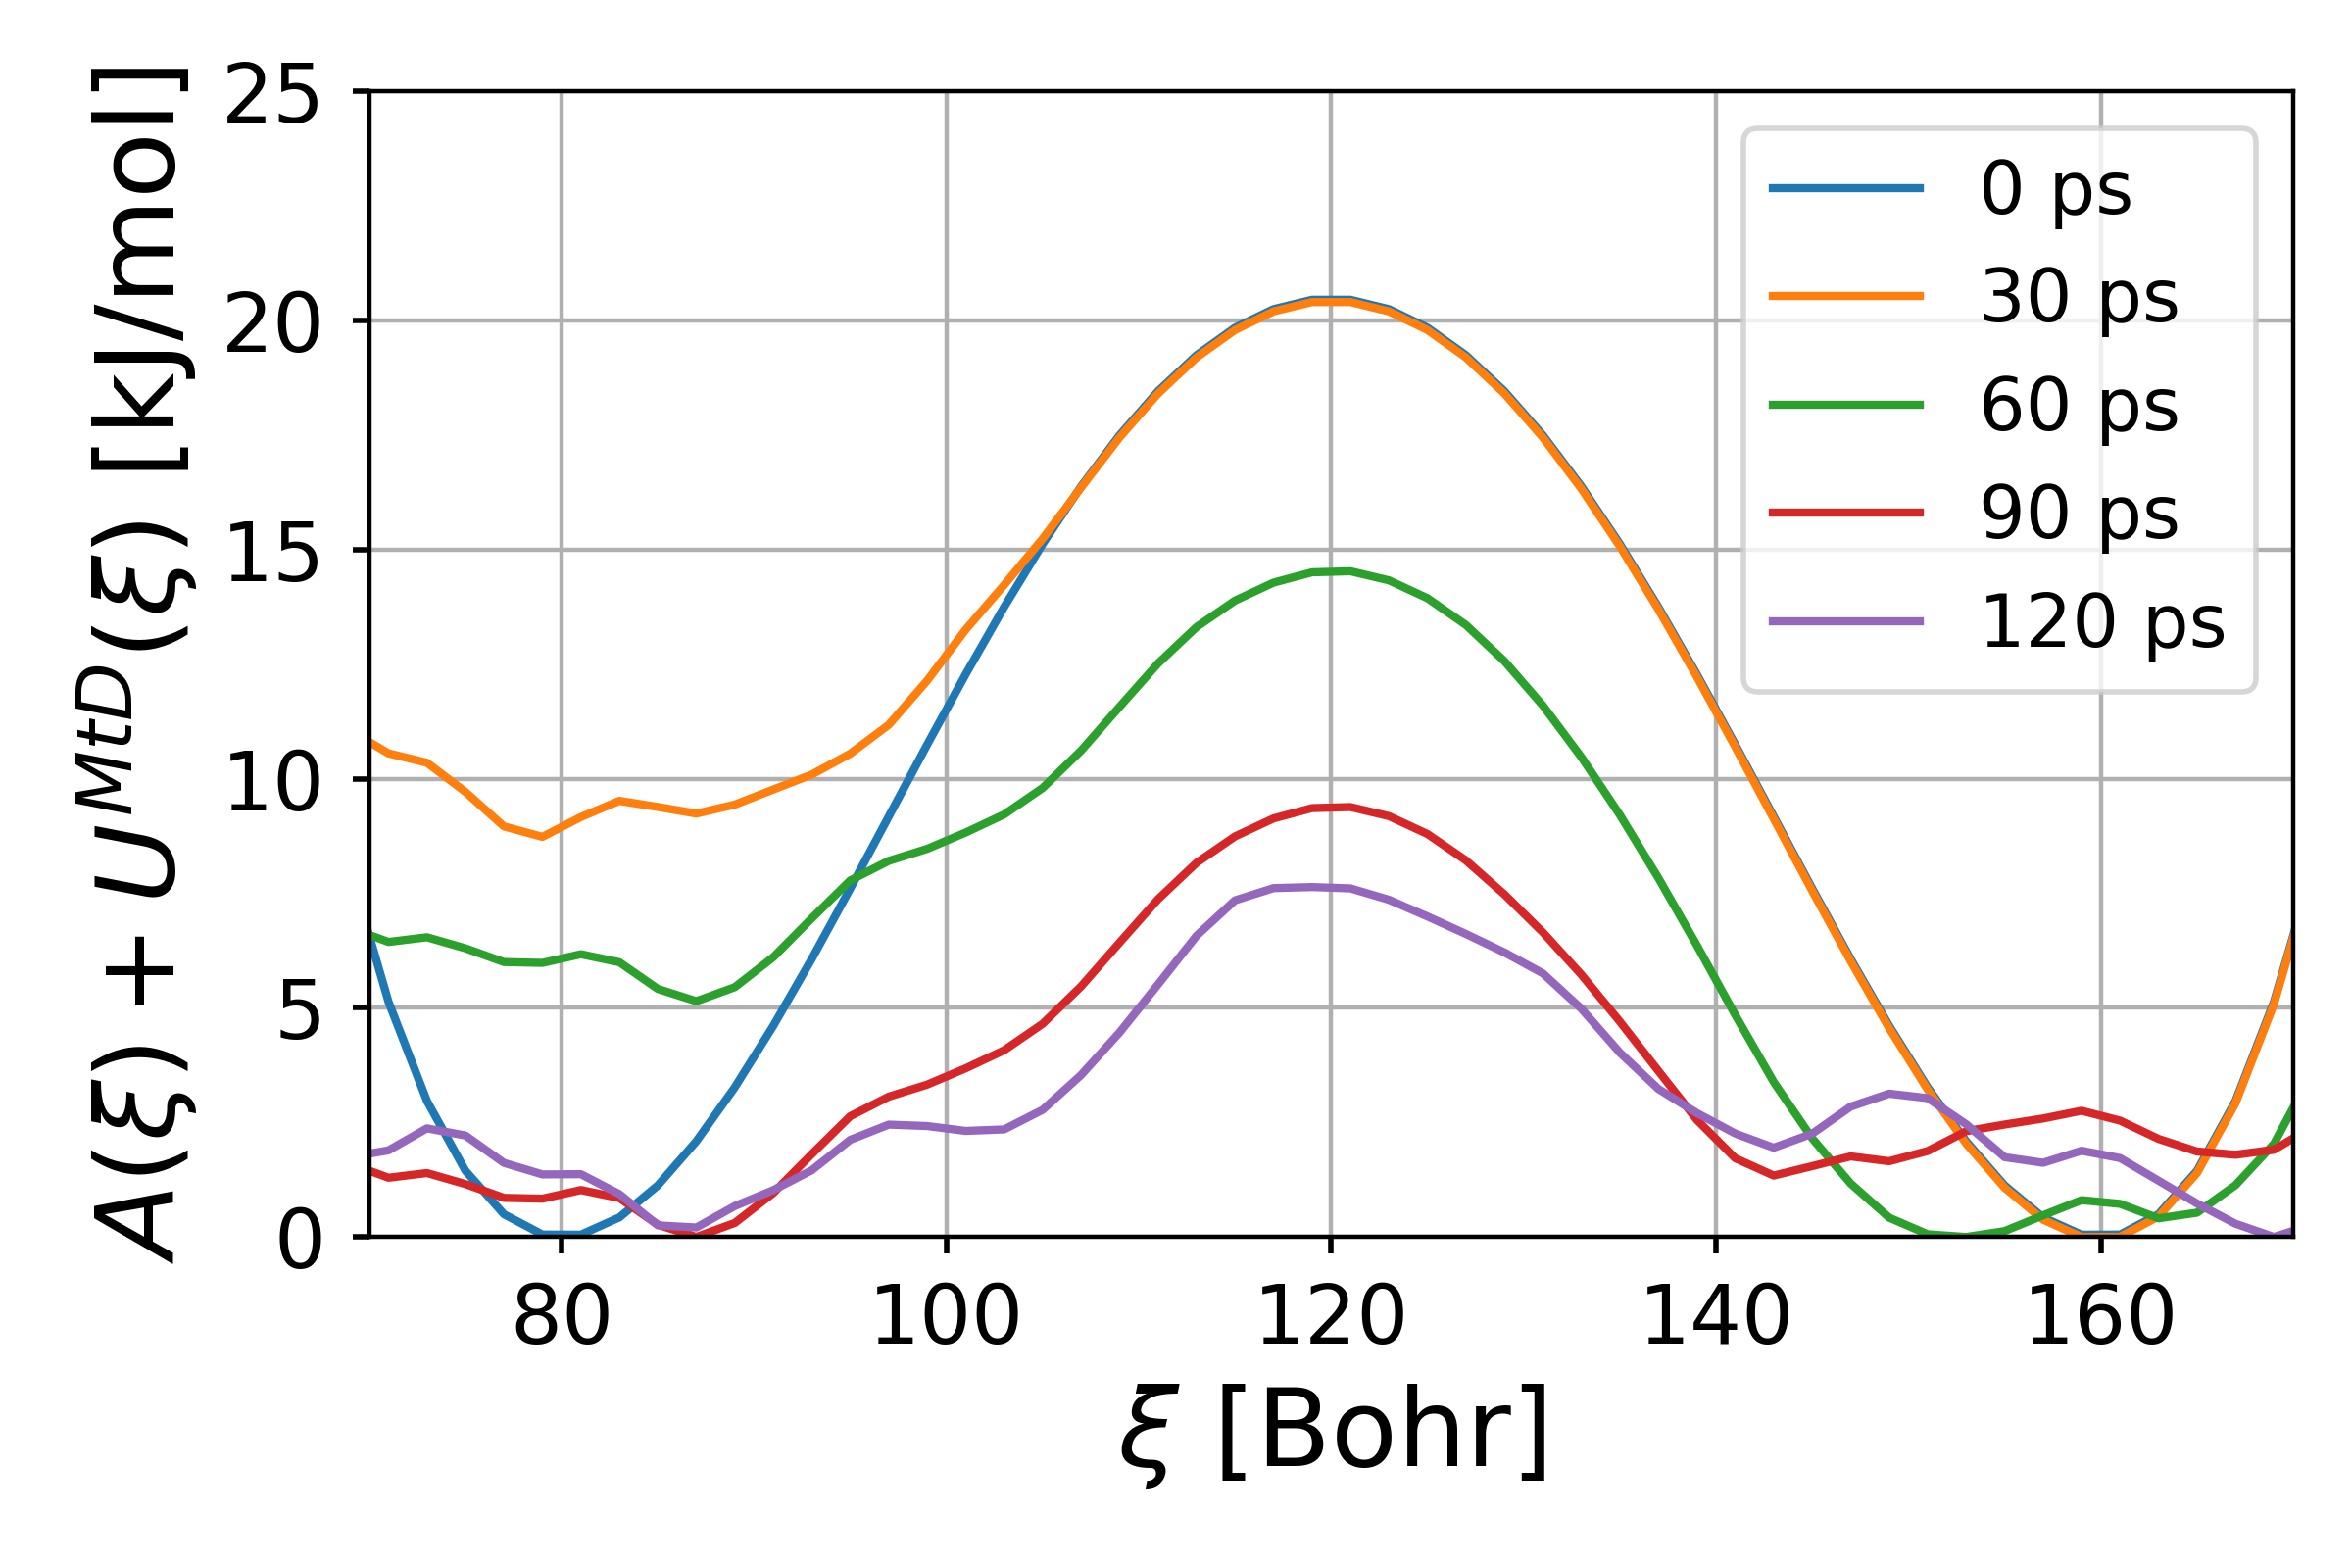
\includegraphics[width=0.49\textwidth]{bilder/metaD_eff_pot} }}
    \subfloat[Well-Tempered Metadynamics]{{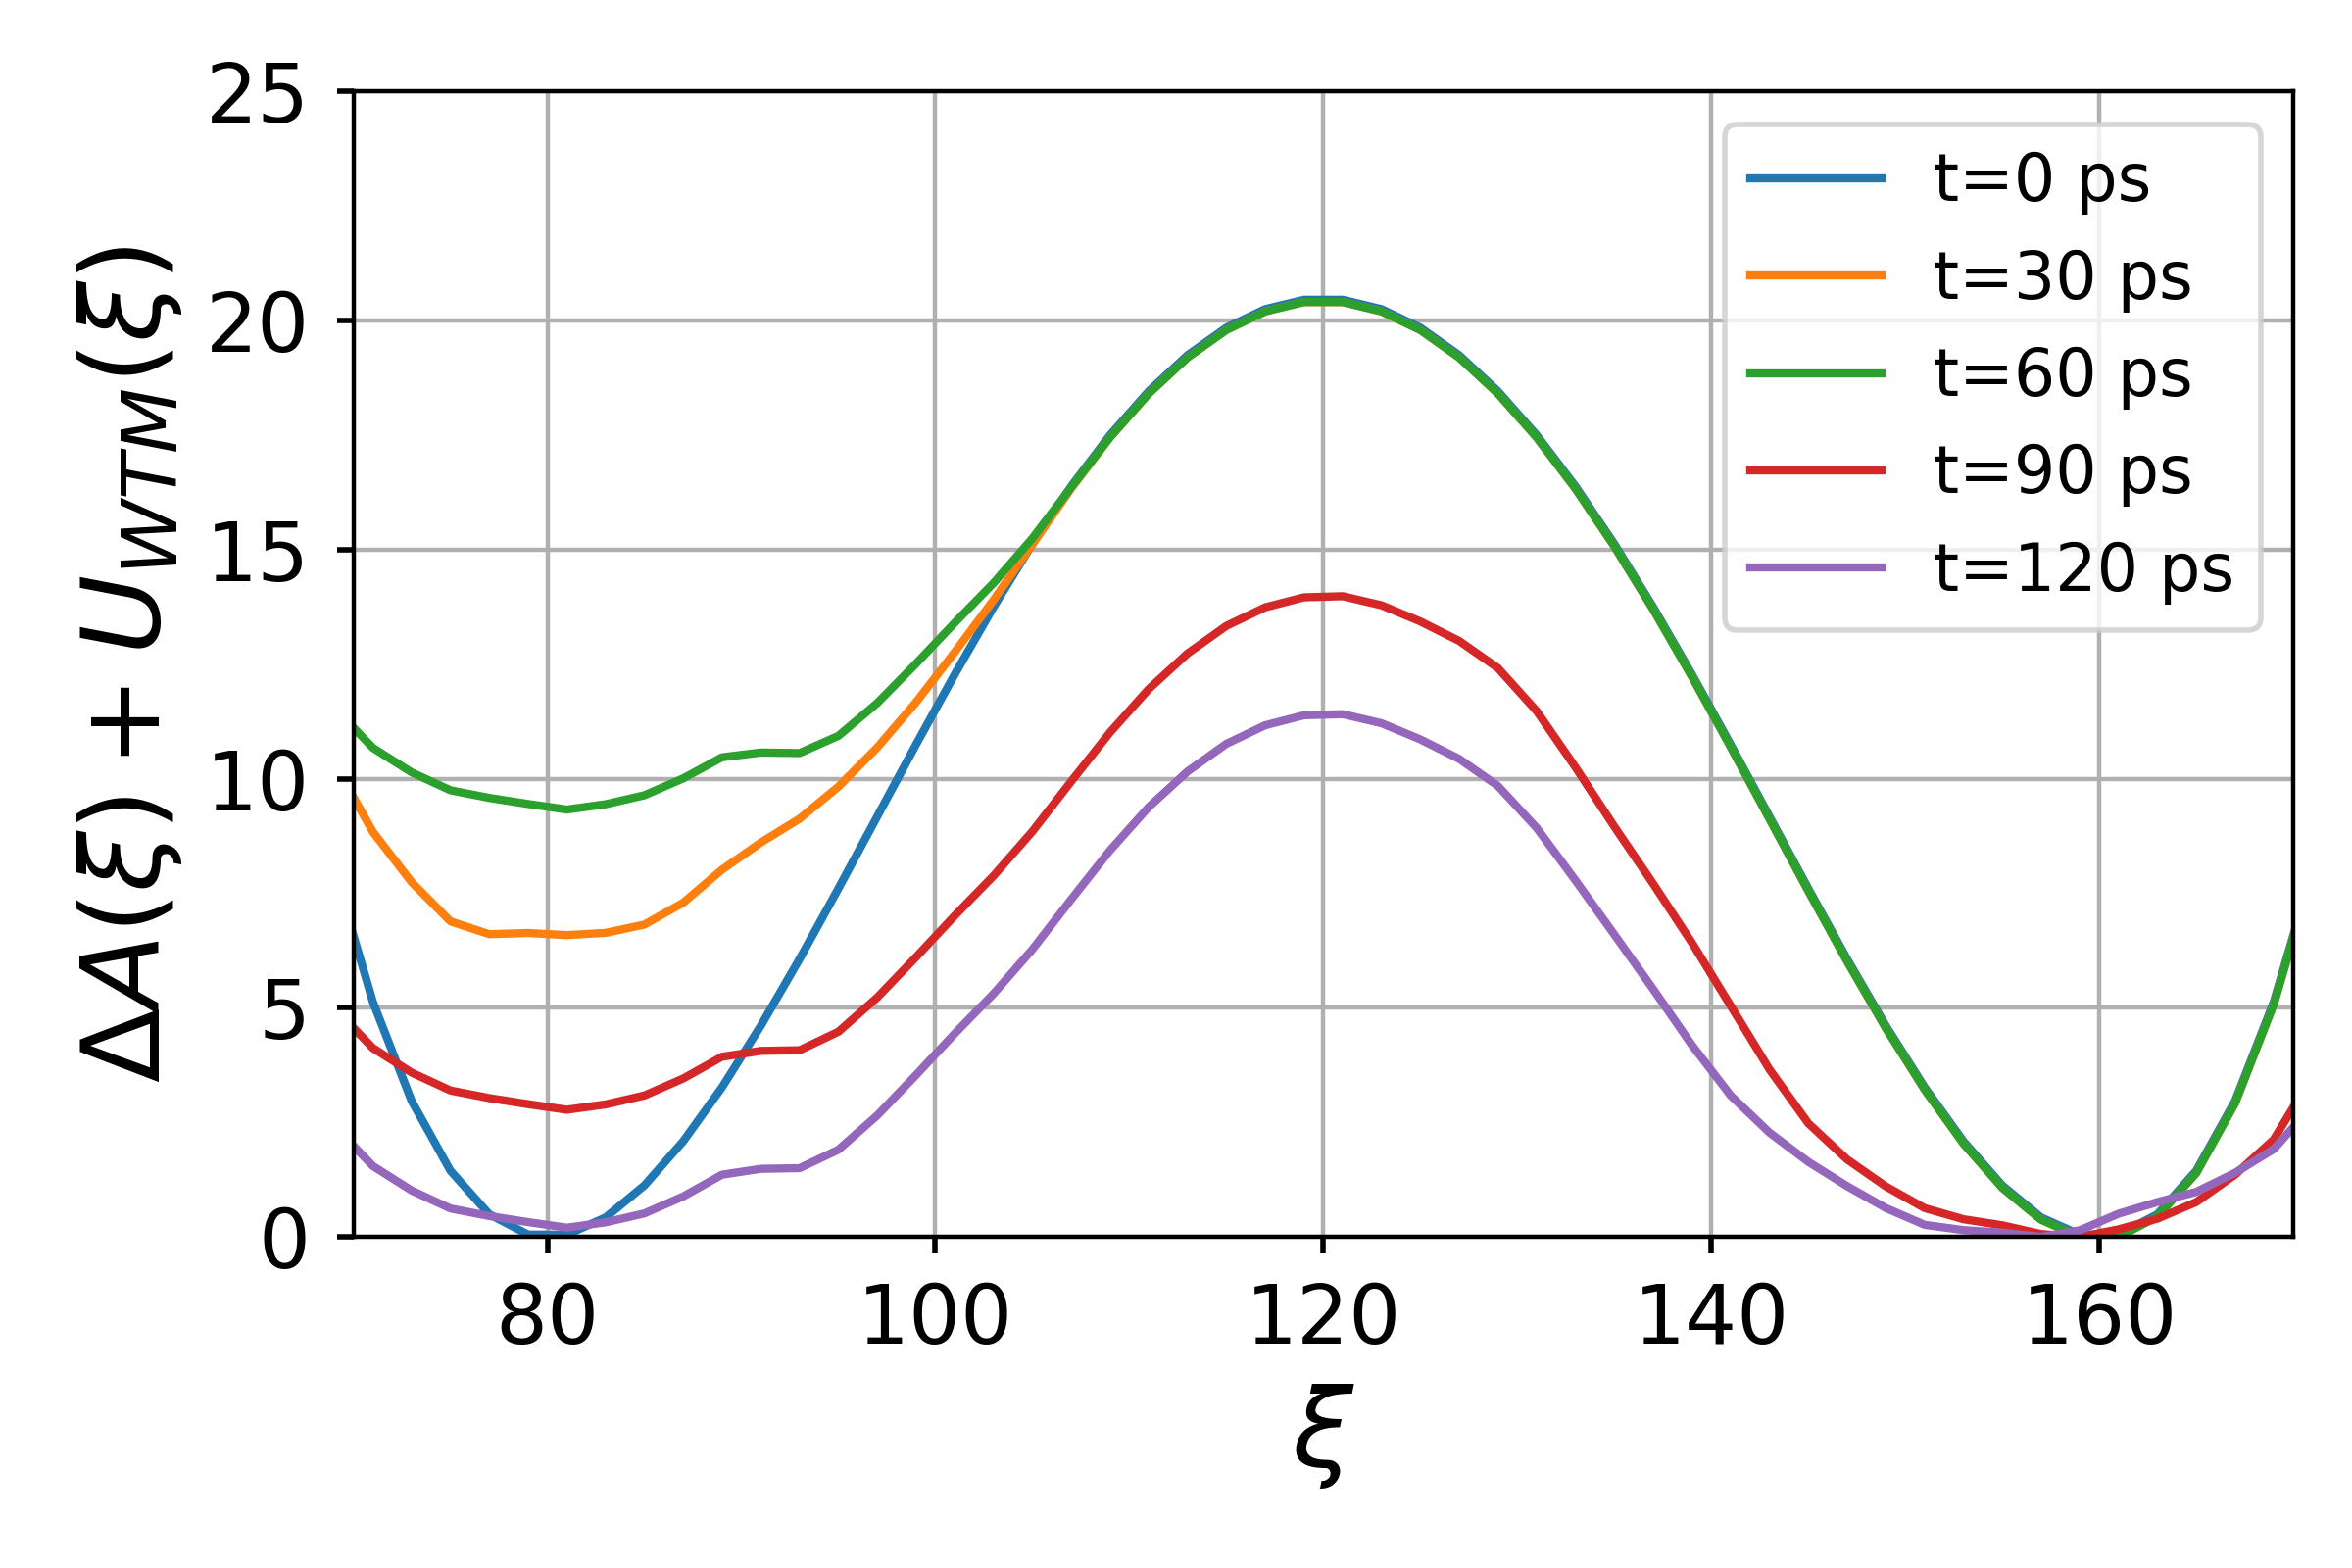
\includegraphics[width=0.49\textwidth]{bilder/WTM_eff_pot} }}
    \caption{Numerical example of the metaD and WTM algorithm for a particle in a 2D double well potential. The reaction coordinate $\xi$ is the x-direction. Over time the bias potentials $U^{MtD}$ and $U^{WTM}$ build up and reduce the free energy barrier. $U^{MtD}$ will ultimately completely remove the free energy barrier, whereas $U^{WTM}$ converges to a certain limit, which can be controlled with parameter $\Delta T$. Details are given in the Appendix.}
\label{fig:metaD}%
\end{figure}

\newpage
\subsection{Adaptive Biasing Force Method (ABF)}
\label{sec:ABF}

The intuition behind ABF is, that if one would know the derivative of the PMF, adding a force $\frac{\partial A(\textbf{x})}{\partial \xi}\nabla\xi(\textbf{x})$ would exactly compensate the average of the original force $-\nabla U(\textbf{x})$ along a given coordinate and result in uniform sampling along this coordinate.\autocite{comer2015adaptive}
Historically, this idea emerged from thermodynamic integration (TI), were the free energy derivative  is computed as the ensemble average of instantaneous force samples, $F$, acting along the collective variable:
\begin{equation}
\frac{dA}{d\xi} = -\braket{F}_{\xi}
\end{equation}
and the PMF is calculated as the integral over this force.\autocite{kirkwood1935statistical,zwanzig1954high}
In practice, as one has no prior knowledge of the free energy derivative, ABF uses an on-the-fly estimate of the mean force. For this purpose the transition coordinate $\xi$, connecting two end points, is divided in $M$ equally spaced bins. The approximation of the bias force $\overline{F}(N^k)$ in bin $k$ is the average of collected force samples:\autocite{comer2015adaptive}
\begin{equation}
  \overline{F}(N^k) = \frac{1}{N^{k}} \sum_{\mu=1}^{N^{k}} F_{\mu}^{k}
  \label{eq:mean force}
\end{equation}
At the beginning of the simulation $\overline{F}$ is scaled up by a linear ramp function $R(N^k)$ to prevent large fluctuations of the force estimate from driving the system away from thermal equilibrium.\autocite{comer2015adaptive}
\begin{equation}
  R(N^k)=\left\{\begin{array}{ll} N^k/N_{full}, & N^{k} < N_{full} \\
                                             1, & N^{k} \geq  N_{full}
                \end{array}\right.
  \label{eq:ramp}
\end{equation}
The number of samples when the full biasing force is applied, $N_{full}$, and the bin size are the only free parameters.
It can be proven mathematically, that equation \ref{eq:mean force} converges (under some constraints exponentially) to $-dA/d\xi$ for a sufficiently large number of force samples.\autocite{alrachid2015long}
Figure~\ref{fig:ABF} shows a numerical example for the flattening of the reaction coordinate during an ABF simulation.

\begin{figure}[H]
    \centering
    \subfloat[ABF force $\overline{F}$]{{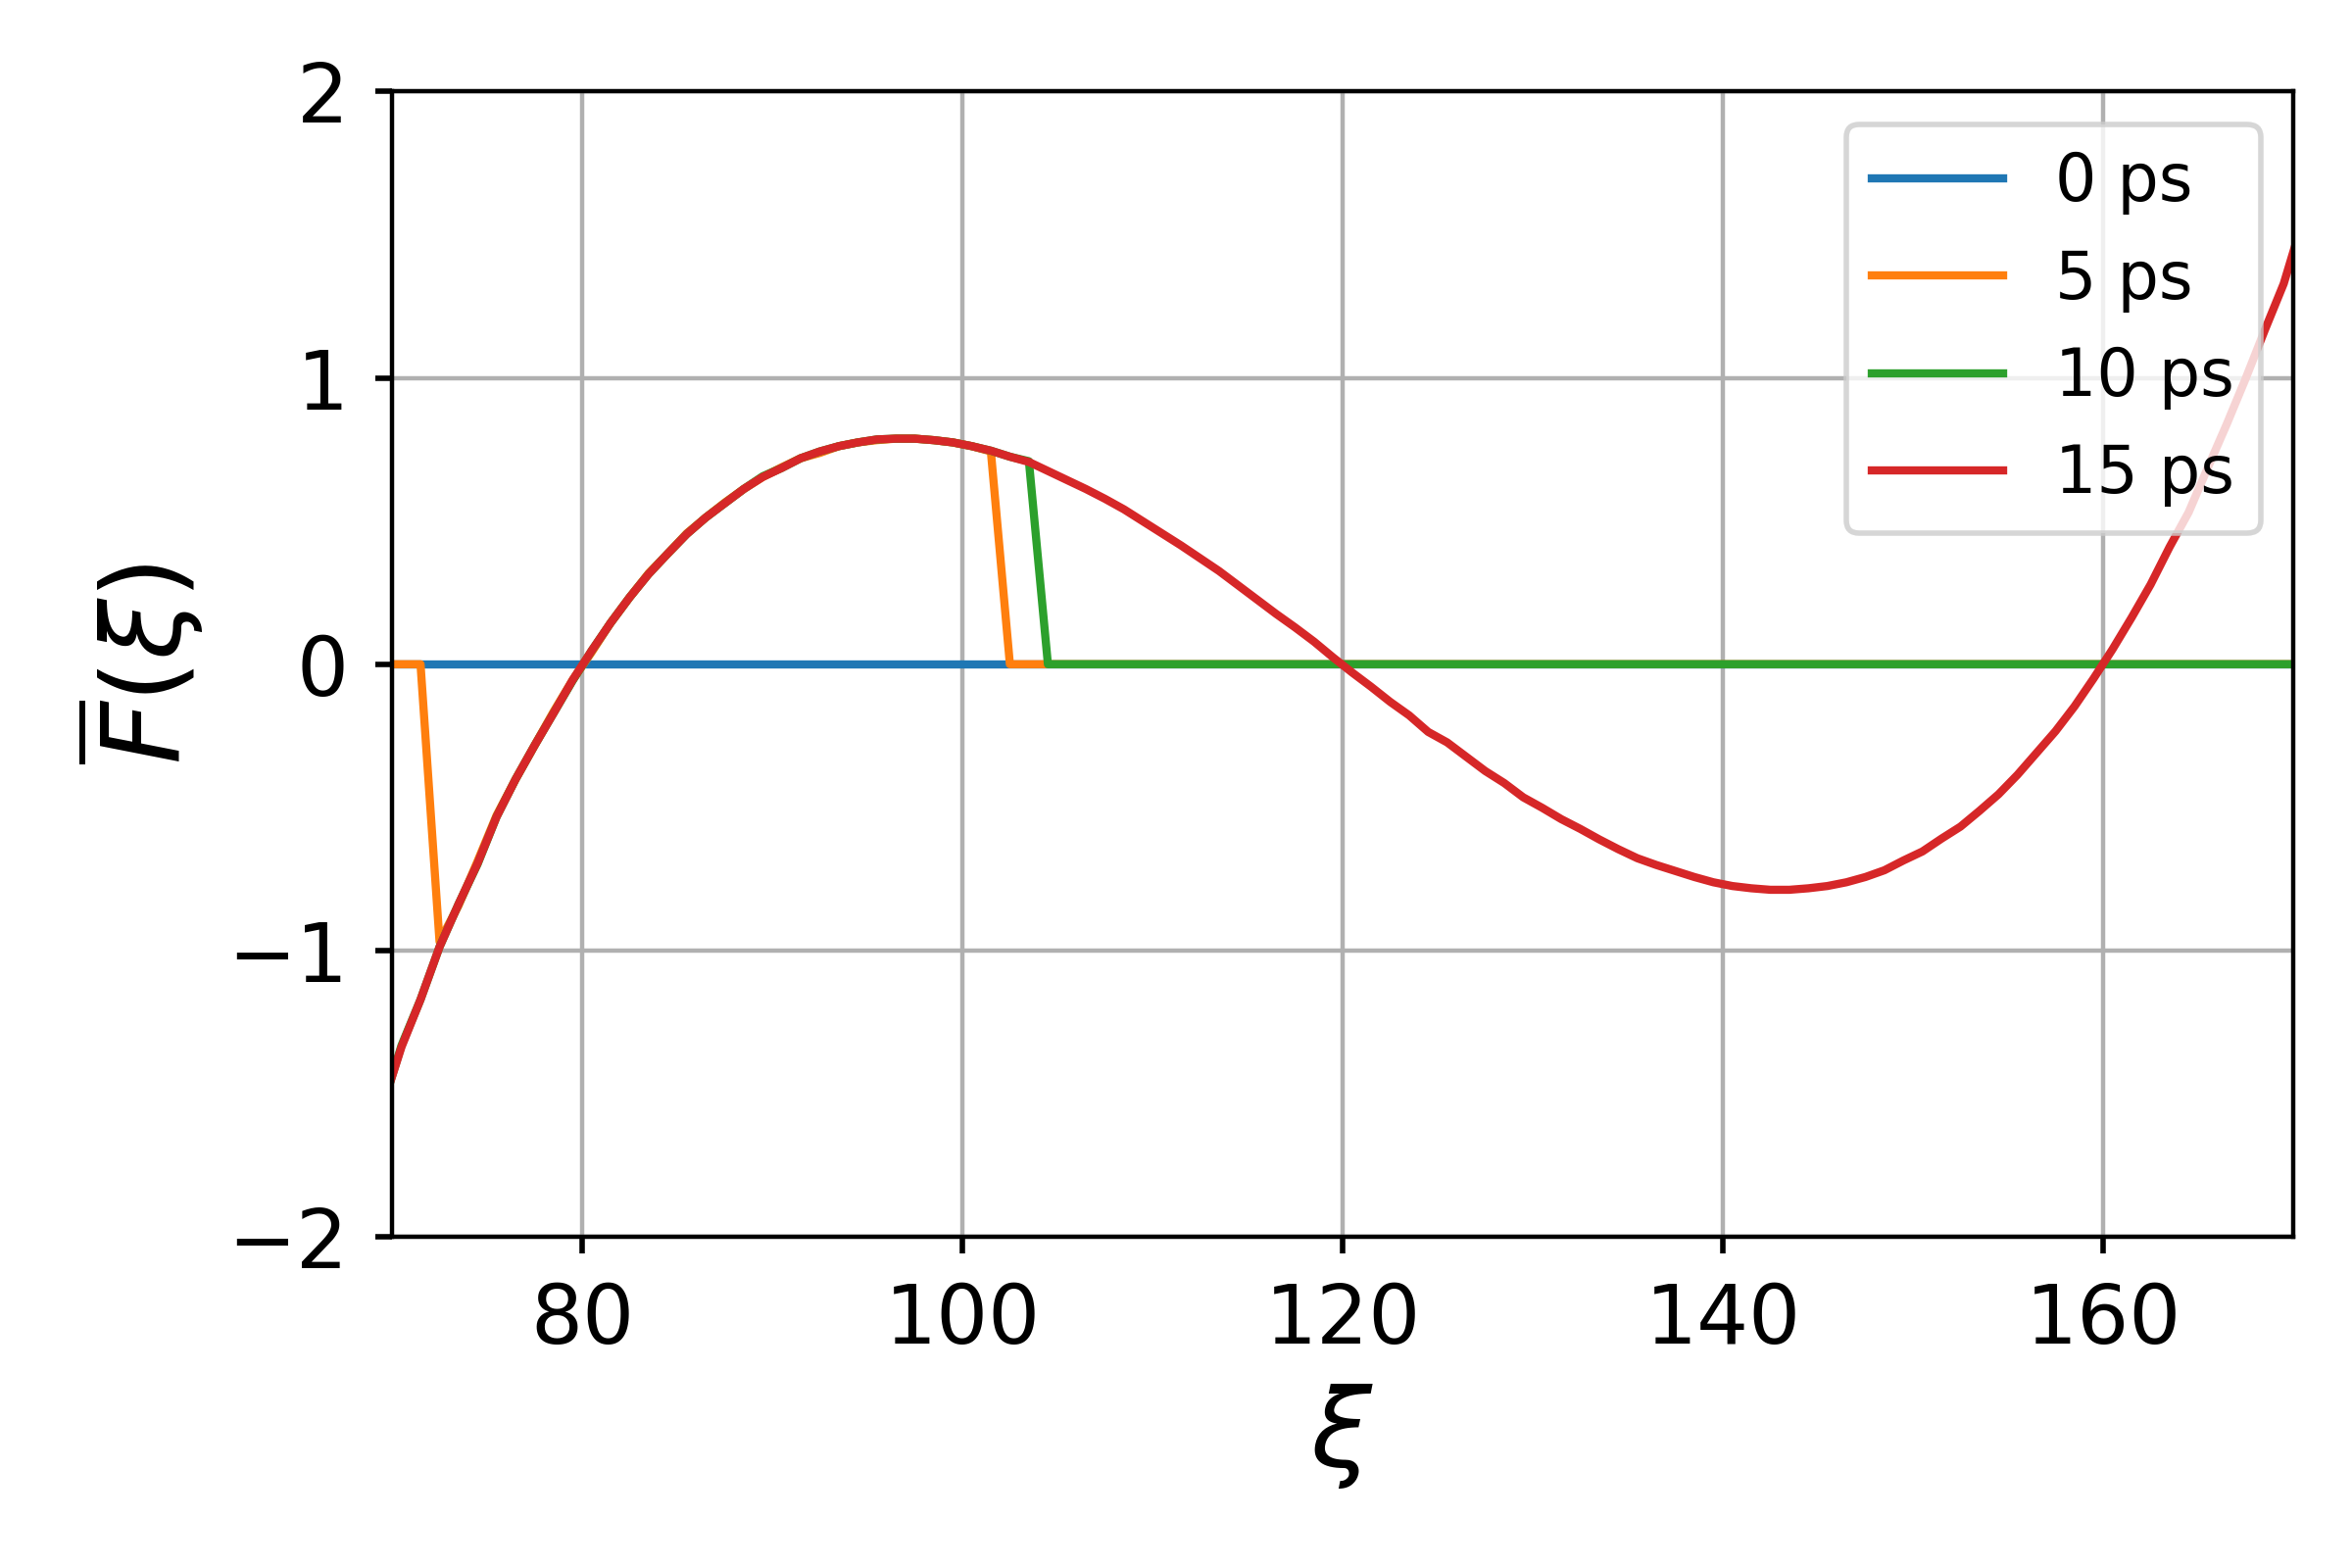
\includegraphics[width=0.49\textwidth]{bilder/ABF_force} }}
    \subfloat[effective potential ($A(\xi)-\int\overline{F}(\xi)d\xi$)]{{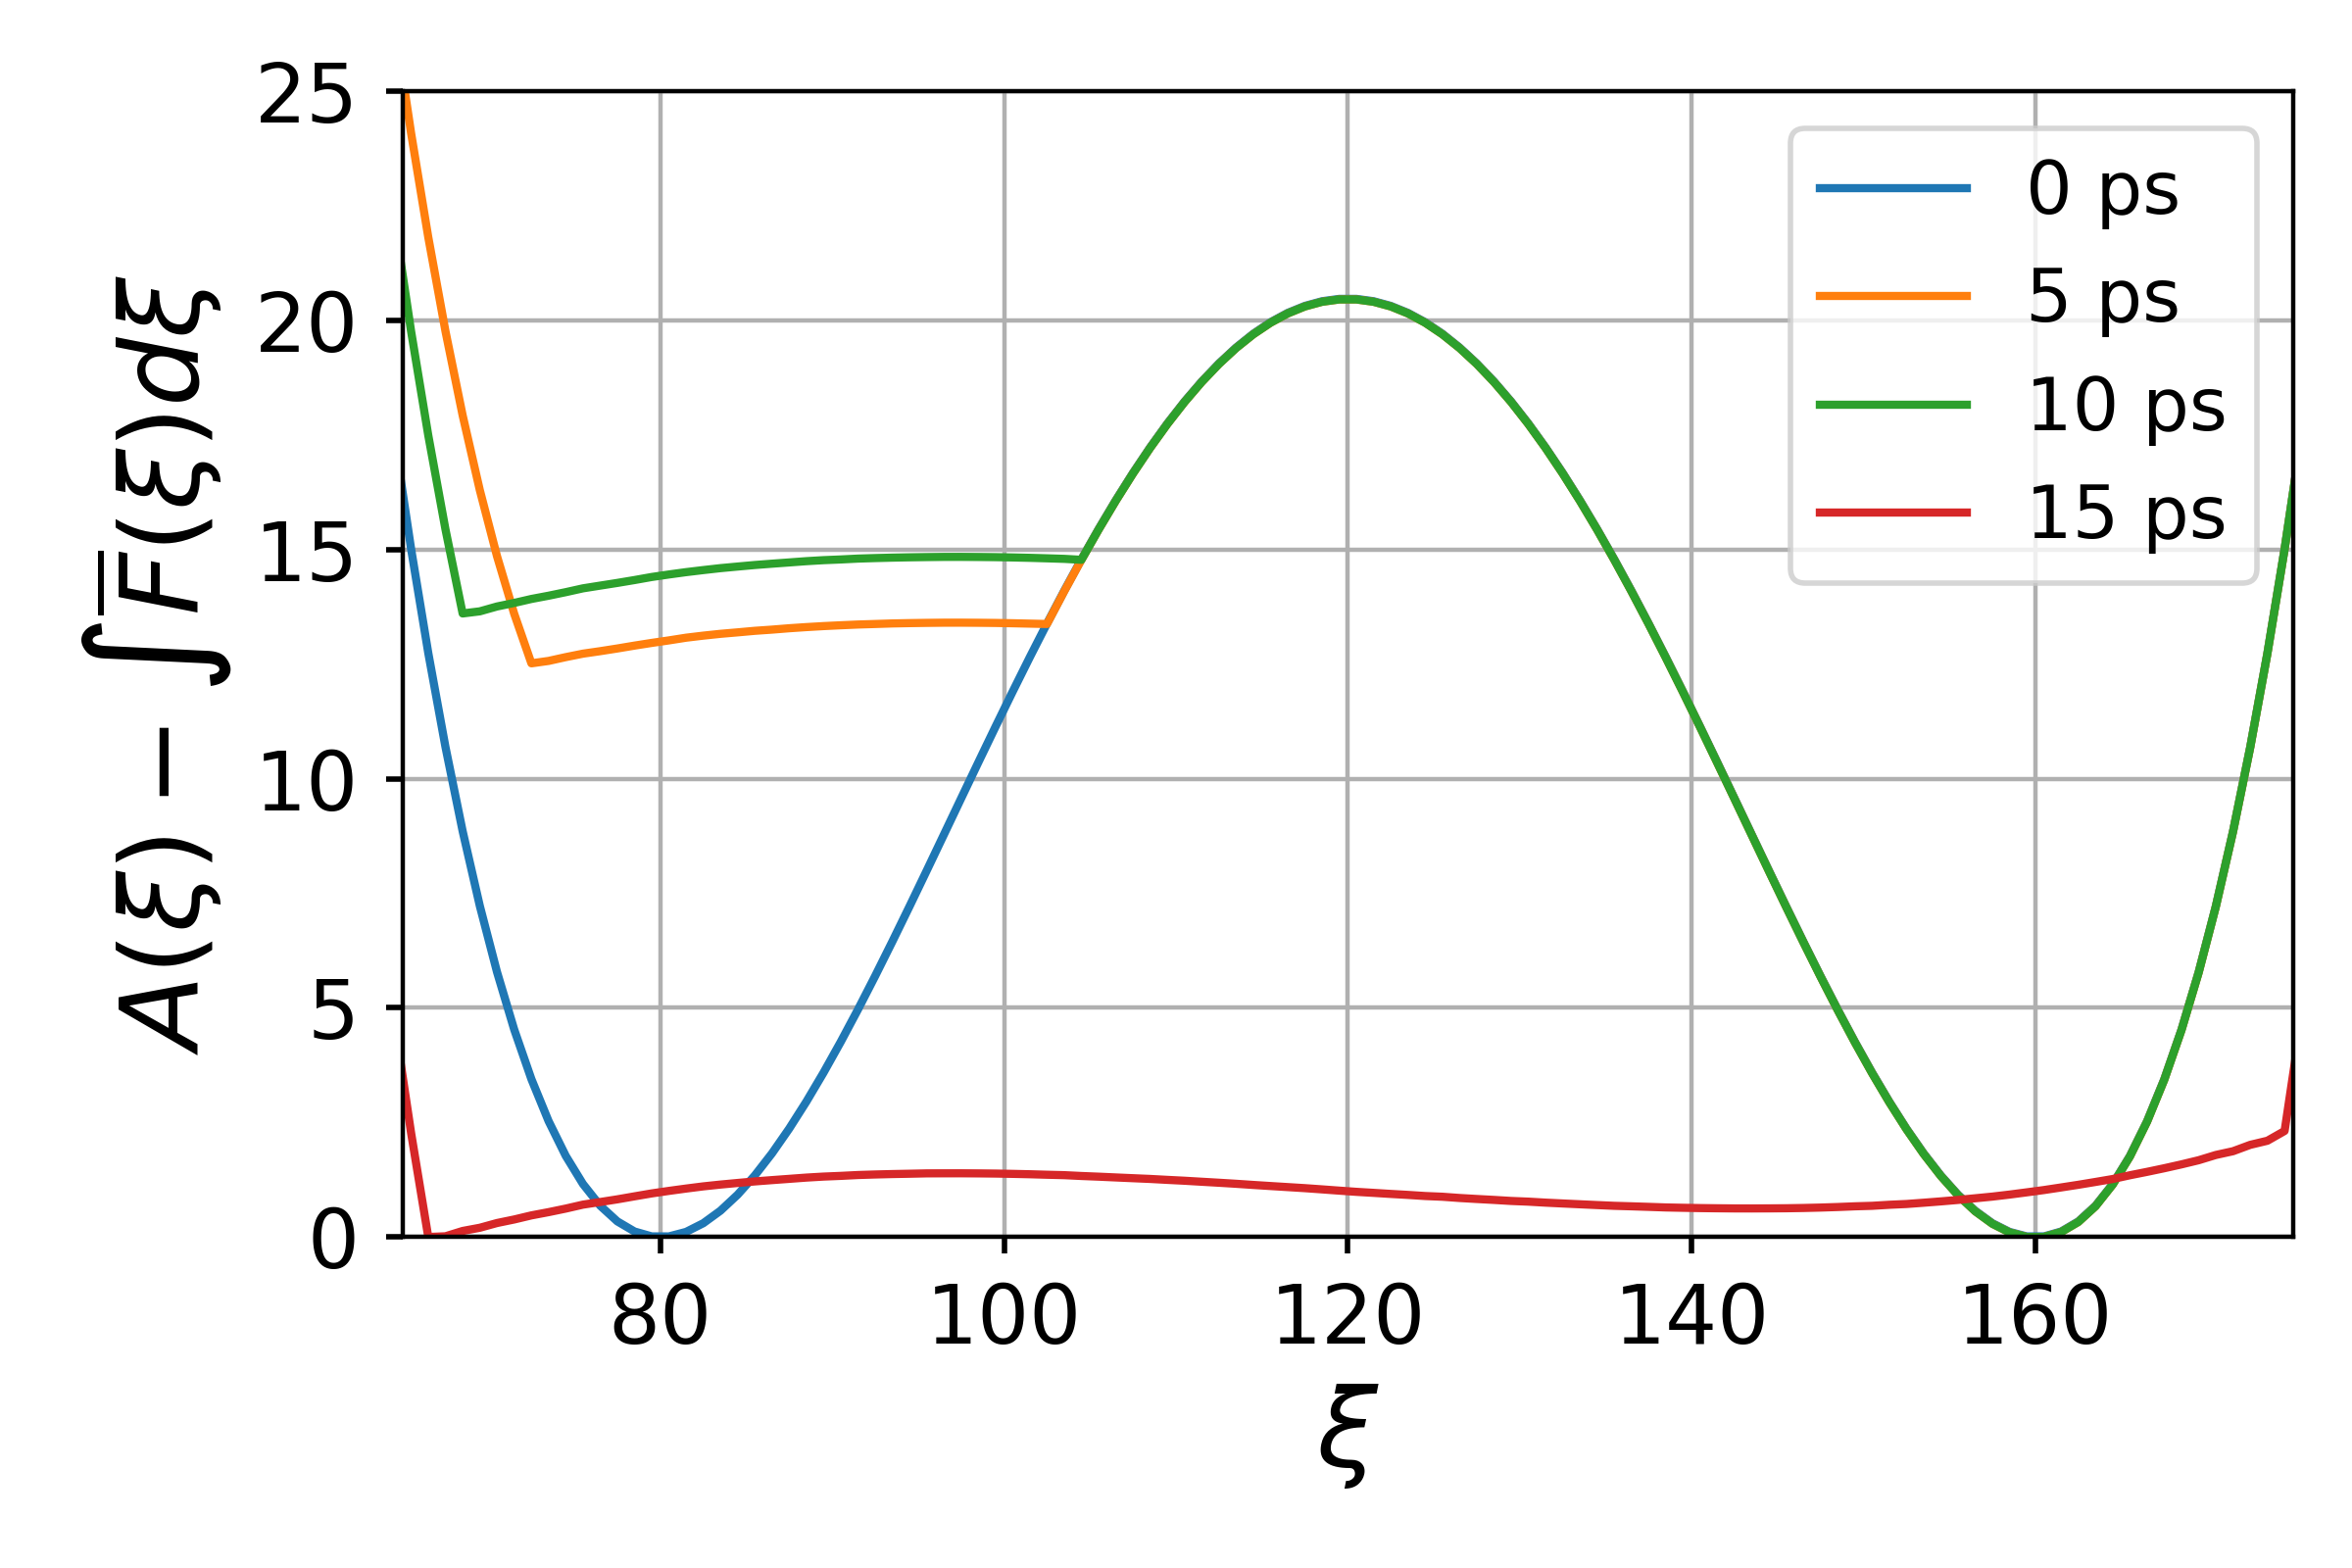
\includegraphics[width=0.49\textwidth]{bilder/ABF_freeE} }}
    \caption{Numerical example of ABF algorithm for a 2D double well potential. The reaction coordinate $\xi$ is the x-direction. $\overline{F}(\xi)$ completely compensates the free energy barrier after 15~ps. From there on, the systems evolution resembles Brownian motion along the flattened reaction coordinate, which will ultimately lead to uniform sampling. Details are given in the Appendix.}
\label{fig:ABF}%
\end{figure}

For 1D reaction coordinates the unbiased free energy difference $A$ can be trivially obtained from $\overline{F}$ with any numerical integration routine.\autocite{davis2007methods}
However, this is not true for two (or higher) dimensional reaction coordinates, because $\overline{F}$ is a non conservative force due to statistical errors.\autocite{comer2015adaptive} With simple integration the result would therefore depend on the integration path, which is physically incorrect. This problem can be avoided by using the \textit{finite element method} (FEM).\autocite{darve2008adaptive} For this purpose in 2D a linear combination of pairwise basis spline (B-spline)\autocite{de1972calculating} functions
\begin{equation}
  B_k(\xi)=\left\{\begin{array}{ll} \frac{\xi-\xi_{k-1}}{\xi_k-\xi_{k-1}}, & \xi \in [\xi_{k-1},\xi_k] \\
                                    \frac{\xi_{k-1}-\xi}{\xi_{k+1}-\xi_{k}}, & \xi \in [\xi_{k},\xi_{k+1}] \\
                                    0, & \text{otherwise}
                  \end{array}\right.
  \label{eq:B spline}
\end{equation}
is used to approximate the PMF.
\begin{equation}
  A(\xi) = \sum_l \alpha_l B_l(\xi). \label{eq:FEM}
\end{equation}
Coefficients $\alpha_l$ are obtained by minimizing the quadratic deviation between force estimates and gradients of spline functions
%\begin{equation}
%  RMSD(\vec{\alpha})=\sqrt{\frac{1}{M}\sum_i^M\biggl(\bigl(\sum_l \alpha_l \nabla B_l(\xi_i)\bigr) - \braket{F(\xi_i)} \biggr)^2}
%  \label{eq:RMSD}
%\end{equation}
\begin{equation}
\text{Error}(\vec{\alpha})=\sum_i^M\biggl|\sum_l \alpha_l \nabla B_l(\xi_i) - \braket{F(\xi_i)} \biggr|^2
  \label{eq:RMSD}
\end{equation}
with the BFGS algorithm\autocite{nocedal2006numerical} for force estimates of all dimensions.\autocite{darve2008adaptive} To increase the smoothness of the reconstructed free energy surface in practice, four control points per bin and dimension are chosen between data points. Force estimates for the control points are obtained by linear interpolation between original data points. Figure~\ref{fig:FEM} shows illustrative examples for the application of B-spline functions in the FEM method.
\begin{figure}[H]
    \centering
    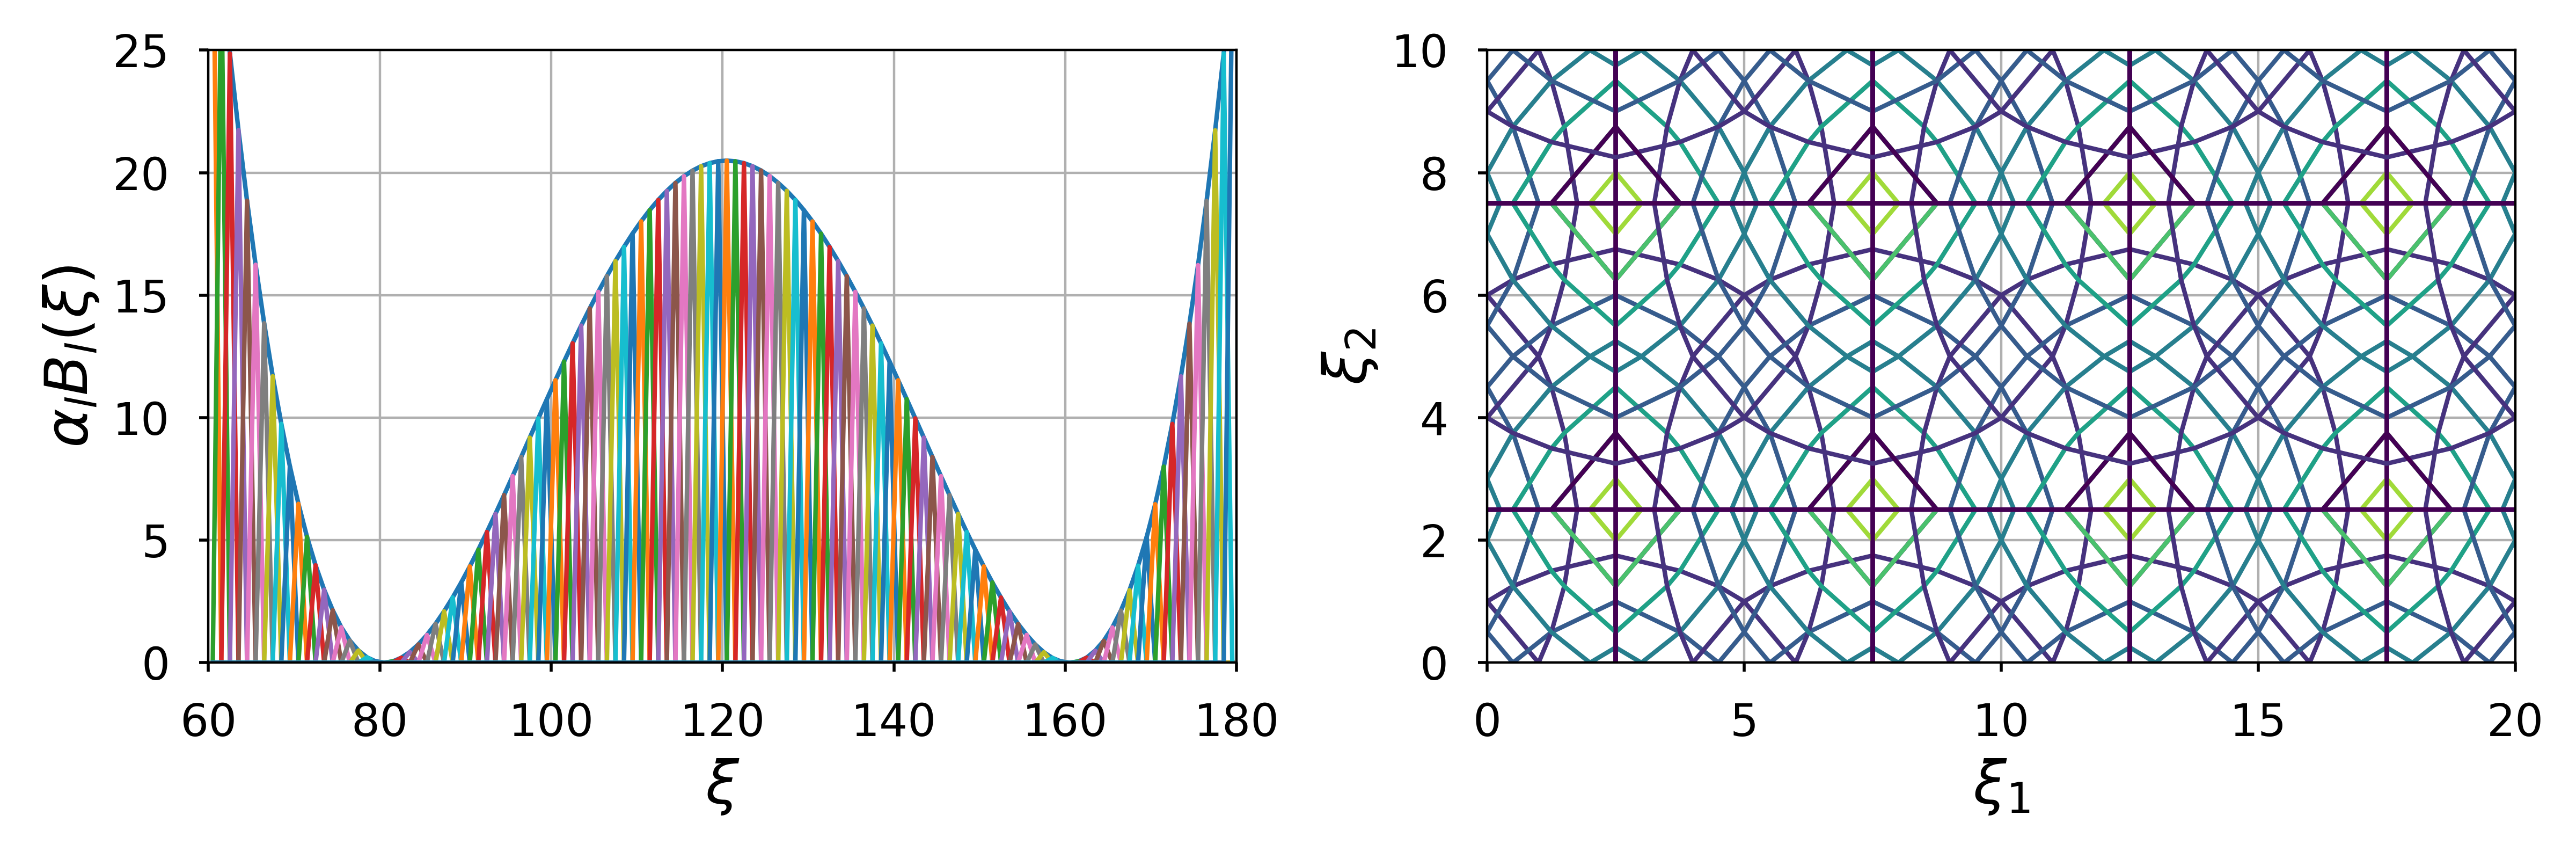
\includegraphics[width=1\textwidth]{bilder/FEM}
    \caption{
      On the left an example for the approximation of an 1D PMF by triangular B-spline functions is shown.
      Right: Illustration of B-spline functions used for integration of 2D ABF data. On each data point one pyramidal B-spline function is centered. Numerically, equation~\ref{eq:RMSD} is evaluated on a grid with four control points per dim and dimension.
    }
\label{fig:FEM}%
\end{figure}
The last missing ingredient for the ABF method is an explicit expression for the instantaneous force samples $F$. Carter et al.\autocite{carter1989constrained} gave a first general expression:
\begin{equation}
  F(\xi,\textbf{q}) = -\frac{\partial U(\xi,\textbf{q})}{\partial \xi} + \beta^{-1} \frac{\partial \ln|J(\xi,\textbf{q})|}{\partial\xi} \label{eq:instforce old}
\end{equation}
which depends implicitly on a vector field $\partial \textbf{x} / \partial \xi$, hereafter referred to as "inverse gradient" and on a Jacobian correction term purely geometric in origin. The inverse gradient can be thought of as the direction along which an infinitesimal change in $\xi$ is propagated in cartesian coordinates keeping complementary coordinates $\textbf{q}$ constant. A major drawback of this formalism is the requirement of a full coordinate transform from cartesian coordinates ($\textbf{x}$) to generalized coordinates ($\xi$, $\textbf{q}$).

This requirement was lifted in work by den Otter\autocite{den2000thermodynamic}, who put forward the idea that the change in $\xi$ can be propagated along an arbitrary vector field $\textbf{v}_i$ ($\mathbb{R}^{3N} \to \mathbb{R}^{3N}$), provided it satisfies some orthonormality conditions.
Extended to multidimensional reaction coordinates \textbf{$\xi$} = ($\xi_i$) and in presence of a set of holonomic constraints $\sigma_{k}(\textbf{x})=0$, these read:\autocite{ciccotti2005blue}
\begin{equation}
  \textbf{v}_i \cdot \nabla \xi_j = \delta_{ij} \label{eq:cond1}
\end{equation}
\begin{equation}
  \textbf{v}_i \cdot \nabla \sigma_k = 0 \label{eq:cond2}
\end{equation}
If all CVs $\xi_i$ are orthogonal to one another and to all constraints, $\textbf{v}_i = \nabla \xi_i/|\nabla \xi_i|^2$ is always a valid option, but not necessarily the best.
Otherwise conditions \ref{eq:cond1} and \ref{eq:cond2} can be fulfilled by orthogonalization:\autocite{ciccotti2005blue}
\begin{equation}
  \textbf{v}_i (\textbf{x}) = \frac{Q^i \nabla \xi_i (\textbf{x})}{|Q^i \nabla \xi_i (\textbf{x})|^2} \label{eq:ortho v}
\end{equation}
with projector $Q^i$ given by the orthonormal basis $\{\hat{n}|_{j}^{i}(\textbf{x})\}_{j\neq i}$ in the subspace spanned by $\{\nabla \xi_j (\textbf{x})|\}_{j\neq i} \cup \{\nabla\sigma_j (\textbf{x})|\}_{j=1,...,M}$:
\begin{equation}
  Q^i = \textbf{1} - \sum_{j \neq i} \hat{n}_{j}^{i}(\textbf{x}) \otimes \hat{n}_{j}^{i}(\textbf{x})
\end{equation}
Replacing the inverse gradient by vectorfield $\textbf{v}_i$, expression \ref{eq:instforce old} finally reduces to:
\begin{equation}
  F(\xi_i,\textbf{x}) = -\nabla U(\textbf{x}) \cdot \textbf{v}_i(\textbf{x}) + \beta^{-1} \nabla \cdot \textbf{v}_i(\textbf{x}) \label{eq:inst ABF force}
\end{equation}
but still involves the calculation of second derivatives in the form of the divergence of vector fields $\textbf{v}_i$.\autocite{comer2015adaptive} Analytic expressions for distances, projected distances, bond angles, and torsion angles, used in the present work, are given in the appendix. However, for complicated CV's like torsion angles, orthogonalization via equation \ref{eq:ortho v} becomes exceedingly tedious and impractical, significantly limiting the applicability of ABF.

\newpage
\subsection{Extended Lagrangian Based Methods (eABF, meta-eABF, WTM-eABF)}
\label{sec:eABF}
To circumvent the technical requirements of ABF, Lesage et al.\autocite{lesage2017smoothed} proposed a more flexible approach termed extended-system ABF (eABF), where additional coordinates $\lambda_i$ with mass $m_{i}$, which are coupled to reaction coordinates $\xi_i$ with harmonic potentials, are introduced. The extended system ($\textbf{x}$, $\lambda$) evolves according to Langevin dynamics in the potential
\begin{equation}
  U_{ext}(\textbf{x},\lambda) = U(\textbf{x}) + \sum_i^n \frac{(\xi_{i}(\textbf{x})-\lambda_i)^2}{2\sigma_i^2}.
\end{equation}
where the mass $m_i$ of the fictitious particle $i$ and the thermal width between the extended coordinate and physical coordinate $\sigma_i^2=(\beta k_i)^{-1}$ are free parameters.
The key intuition behind eABF is, that in the tight coupling (low $\sigma_i$, high $k_i$) limit, efficient sampling of $\lambda$ will result in efficient sampling of $\xi$.
Therefore, to obtain uniform sampling along $\xi$, it is sufficient to bias the dynamics of $\lambda$. The inverse gradient $\textbf{v}_i$ is chosen as zero for all physical coordinates $\textbf{x}$ and 1 for $\lambda_i$.
In this way constraints \ref{eq:cond1} and \ref{eq:cond2} are always satisfied, which is especially useful for calculations involving a set of non-orthogonal reaction coordinates.
In practice, the Langevin integrator for the extended system is implemented separately from the physical MD engine and can be coupled to any collective variable of interest without additional effort.

Sampling the unbiased extended system in thermal equilibrium gives the following Boltzmann distribution in $\lambda$:
\begin{equation}
  P_\lambda(\lambda) \propto \int \e^{-\beta U_{ext}(\textbf{x},\lambda)} d\textbf{x} \\
\end{equation}
To enhance sampling of the CV the dynamic of $\lambda$ is biased with the ABF algorithm.
The mean force acting on $\lambda$ in bin $k$ is simply given by averaging the harmonic force:
\begin{equation}
  \overline{F}(\lambda_{i}, N^k) = \frac{\partial A^{k}(\lambda_{i})}{\partial \lambda_i} = \frac{1}{N^{k}\sigma_i^2} \sum_{\mu=1}^{N^{k}} (\lambda_{i,\mu}^{k}-\xi_{i,\mu}^{k})
  \label{eq:eABF bias}
\end{equation}
At the beginning of the simulation again the linear ramp function $R(N^k)$ given by equation \ref{eq:ramp} is used.
Note that the force estimate no longer depends on all atomic coordinates $\textbf{x}$ like in normal ABF (cf. equation \ref{eq:inst ABF force}), but only on ($\lambda_i - \xi_i$).
This has the advantageous side effect, that the noise in $\overline{F}$ can be reduced significantly and faster convergence of $\overline{F}$ can be expected, if $\sigma^2$ is well chosen.\autocite{lesage2017smoothed} Specifically, the mean square fluctuation of the spring force is proportional to $(\beta\sigma)^{-1}$, which shows that the variance of $\overline{F}$ is smaller for higher values of $\sigma$.
Over time the biased probability density in $\lambda$ $P^B(\lambda_i)$ given by
\begin{equation}
  \begin{split}
  P^B(\lambda_i) &\propto \int \e^{-\beta U_{ext}(\textbf{x},\lambda_i) +\int \overline{F}(\lambda_{i})d\lambda} d\textbf{x} \\
  &\propto \int \e^{-\beta U_{ext}(\textbf{x},\lambda_i) +A^\lambda(\lambda_{i})} d\textbf{x}
  \end{split}
\end{equation}
will be uniform.
We now need to find a robust estimator to recover the PMF of the original physical system $A(\xi_i)$ from biased dynamics in the extended system.
The naive approach is to approximate $A(\xi_i)$ with $A^\lambda(\lambda_i)$, which is obtained by simply integrating the bias force $\overline{F}(\lambda_{i})$ like in normal ABF.
However, this will only produce unbiased results in the tight coupling limit for $\sigma \rightarrow 0$, where standard ABF is recovered.

An asymptotically unbiased estimator of $A(\xi_i)$ can be derived by correcting the free energy gradient obtained from the eABF-biased distribution $\tilde{p}(\xi)$ with the average biasing force on $\xi$
\begin{equation}
  \begin{split}
\frac{\partial A(\xi_i)}{\partial \xi_i} &= -\beta^{-1}\frac{\partial \ln P^B(\xi_i)}{\partial \xi_i} + k(\braket{\lambda_i}_{\xi_i}-\xi_{i}) \\
  &= -\beta^{-1}\frac{\partial \ln \tilde{p}(\xi_i)}{\partial \xi_i} + \overline{F}_{corr}
\end{split}
  \label{eq:CZAR}
\end{equation}
which is called \textit{Corrected z-averaged restraint} (CZAR)\autocite{lesage2017smoothed} and can be calculated on-the-fly during the simulation at little extra cost by introducing two additional accumulators for $\tilde{p}(z)$ and $k(\braket{\lambda_i}_{z}-z_{i})$ which are only joined at output times. Figure \ref{fig:eABF traj} gives a numerical example for the application of eABF and figure \ref{fig:eABF flowchart} shows a schematic overview of the full eABF/CZAR algorithm.

\begin{figure}[H]
    \centering
    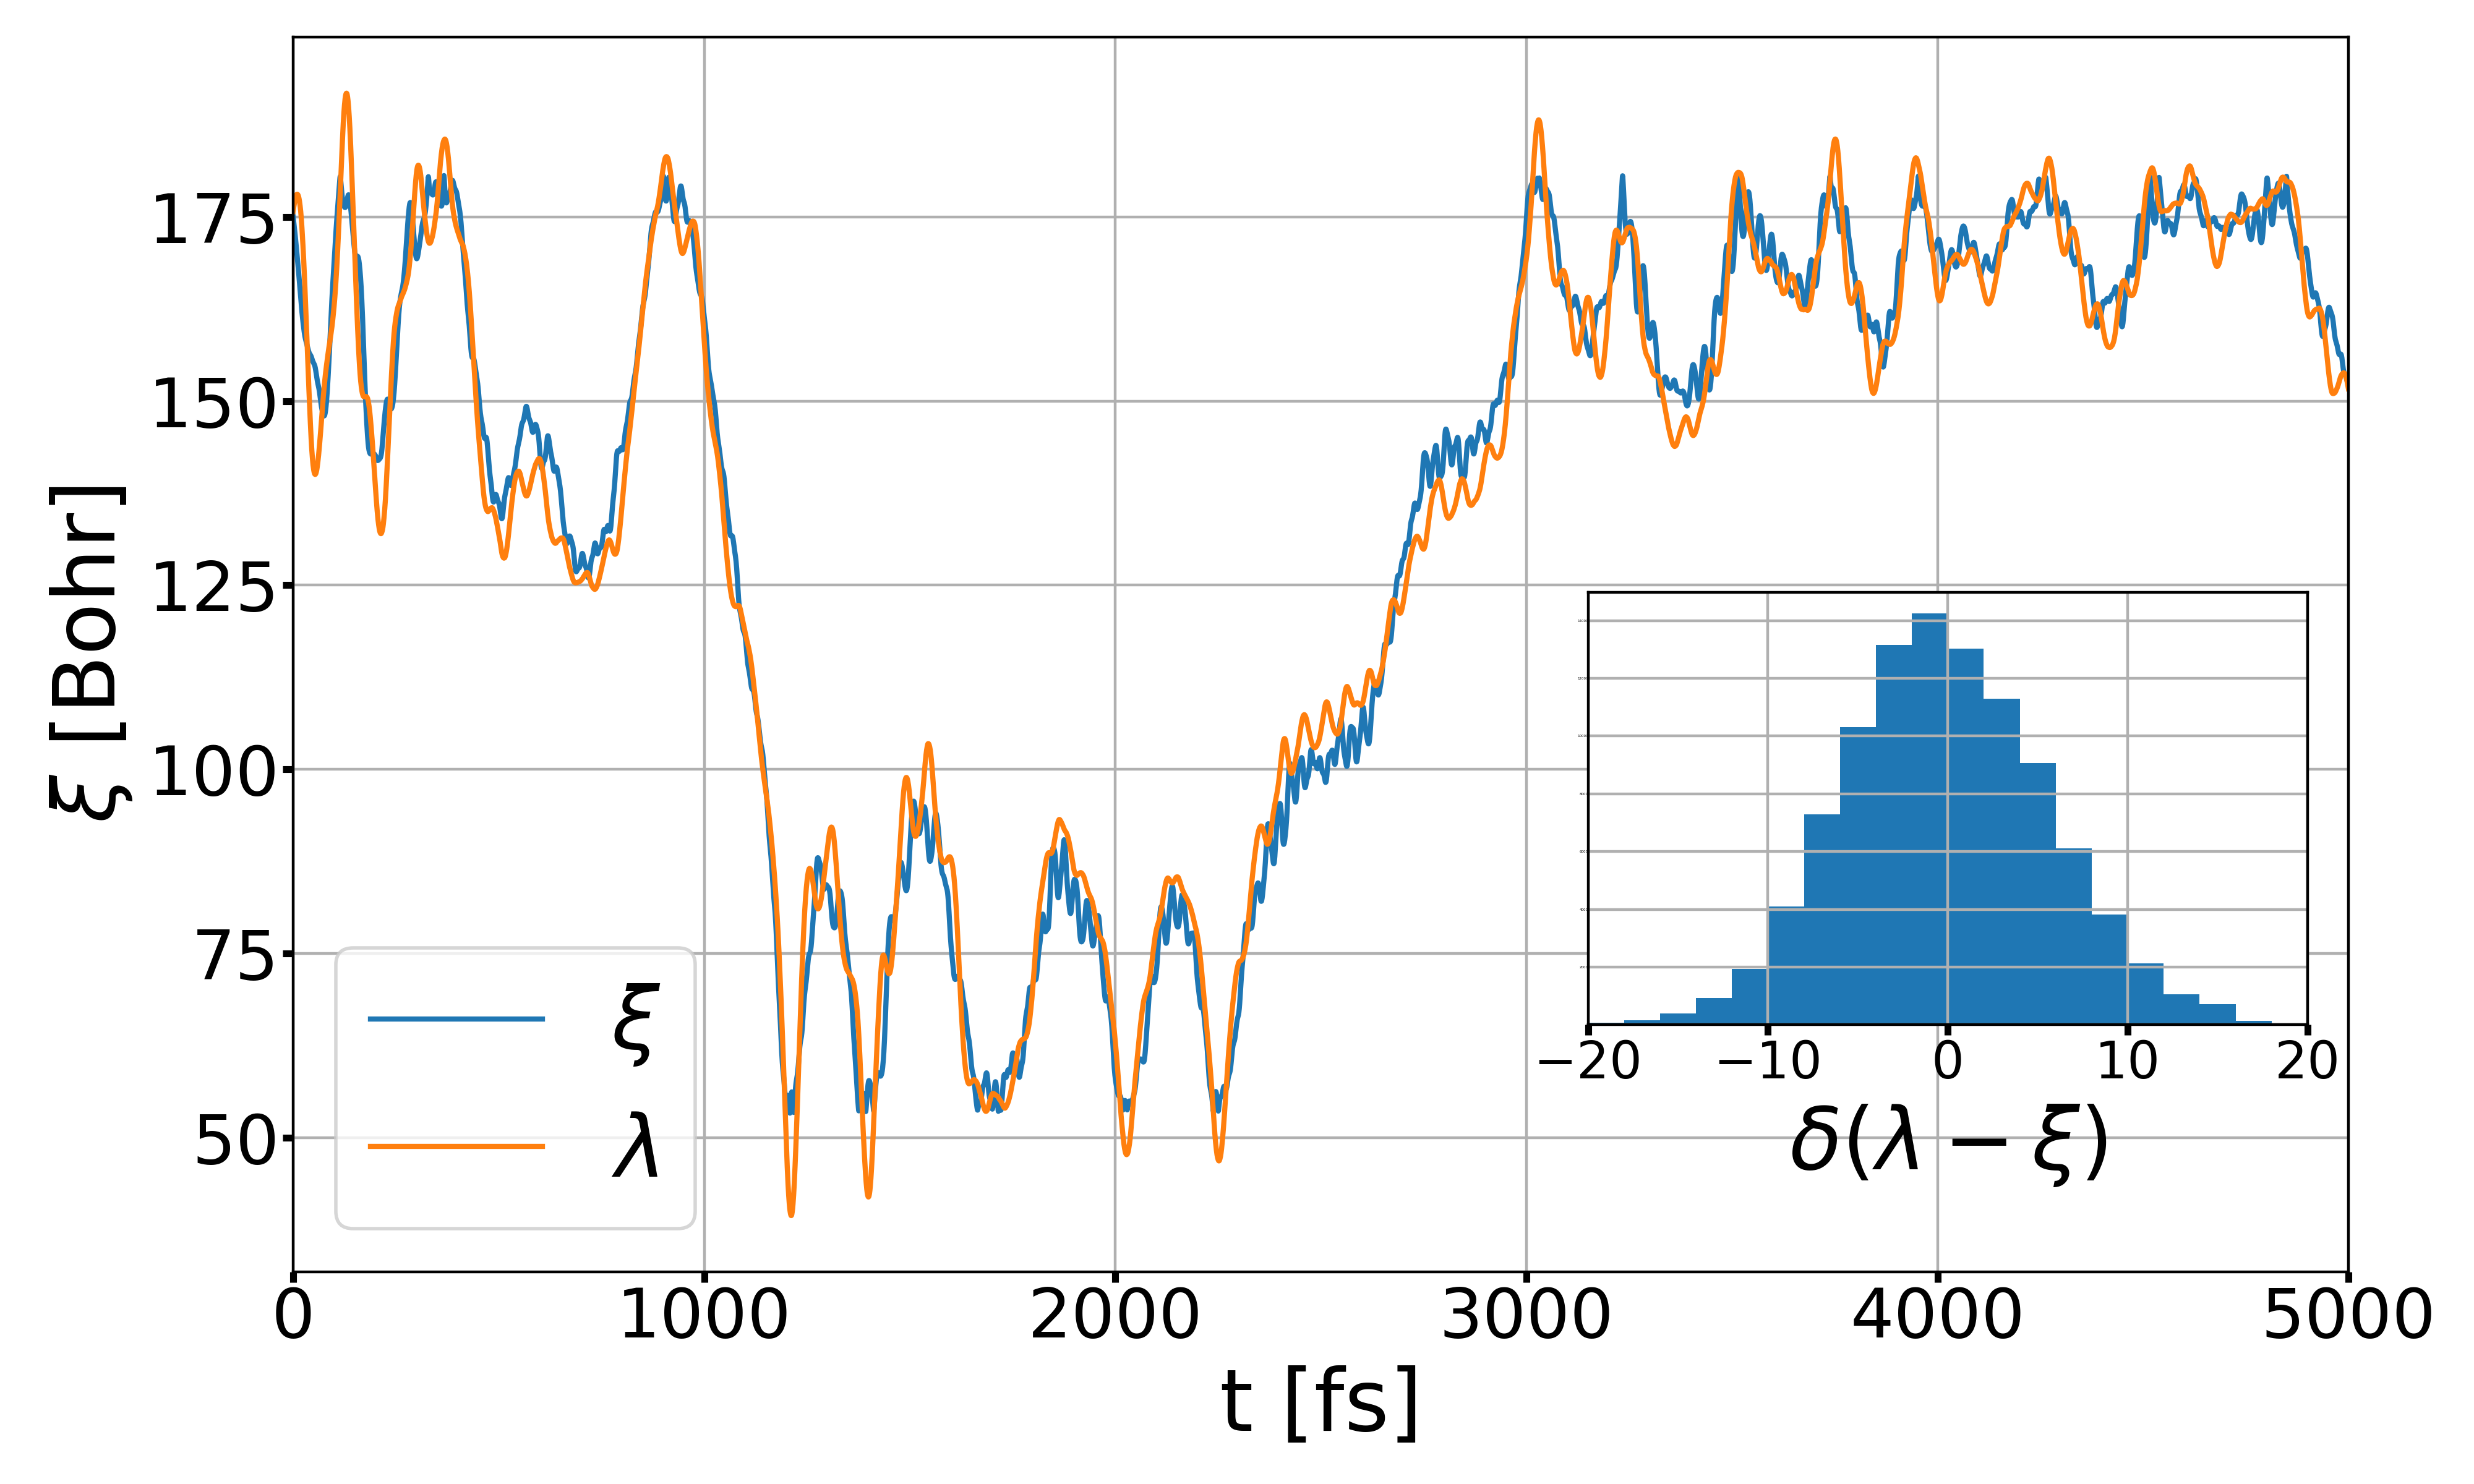
\includegraphics[width=0.49\textwidth]{bilder/eABF_traj}
    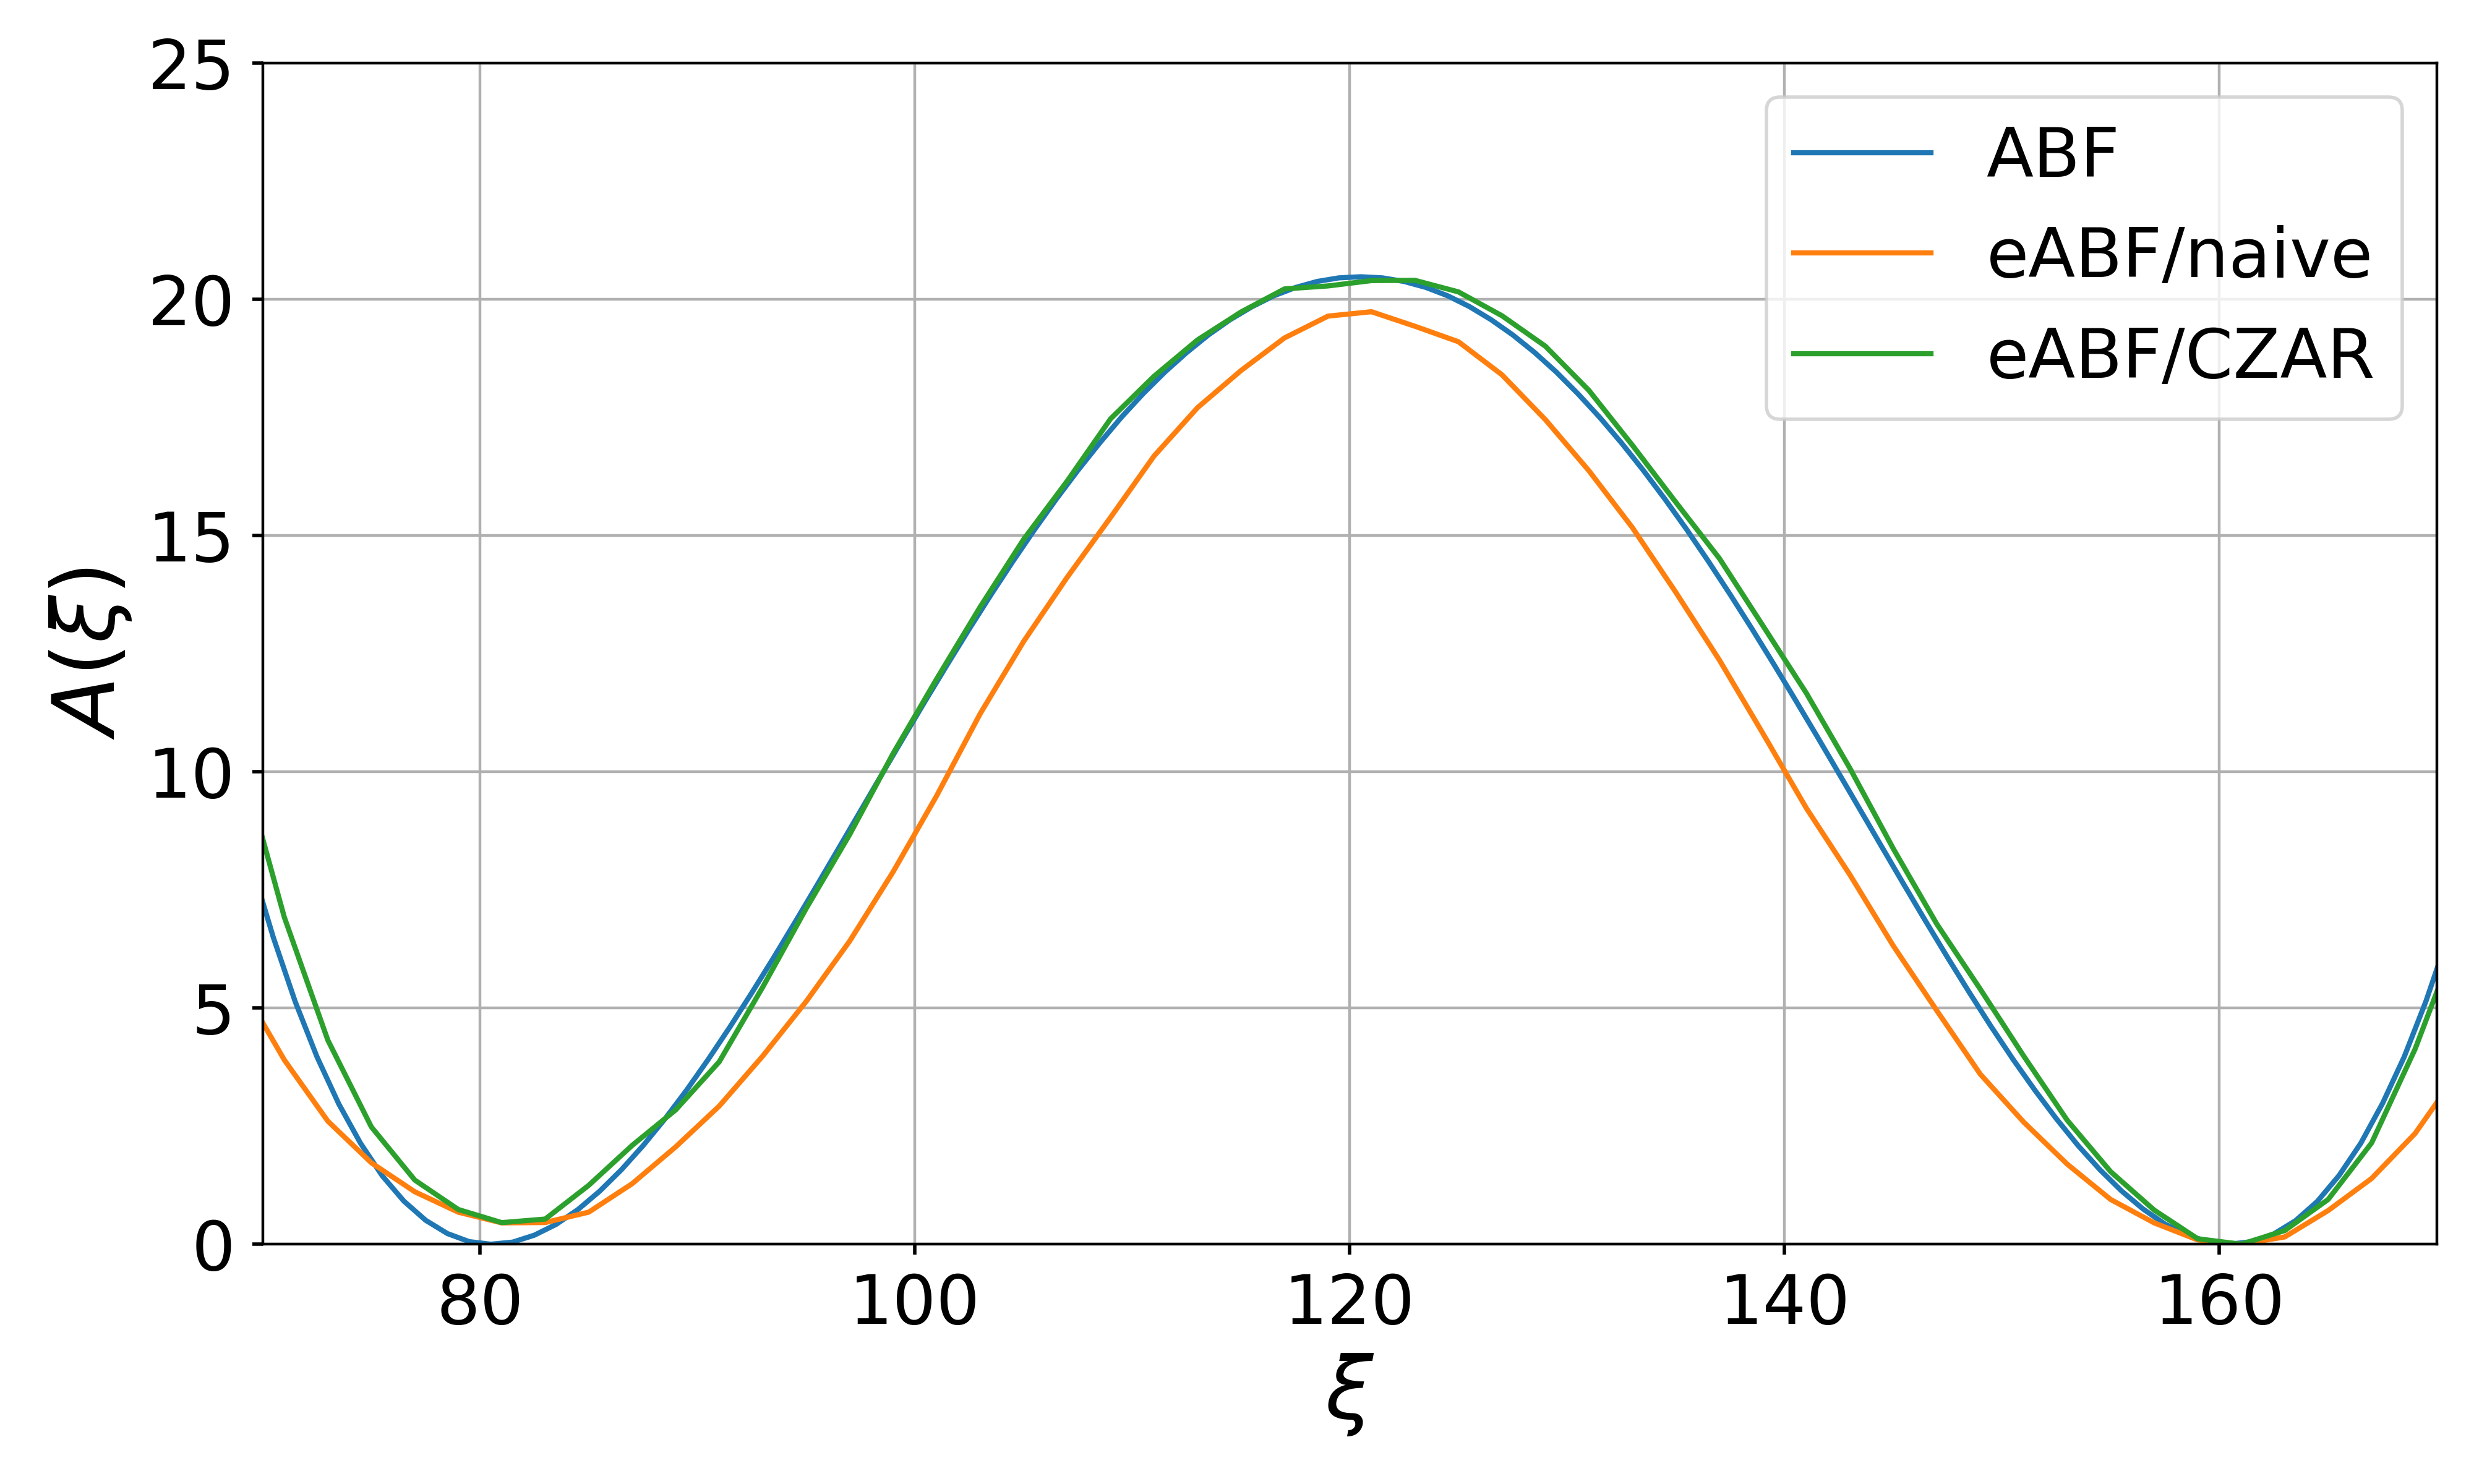
\includegraphics[width=0.49\textwidth]{bilder/eABF_freeE}
    \caption{Numerical examples for eABF algorithm with $m_\lambda=20$~a.u. and $\sigma=7$~Bohr. The reaction coordinate $\xi$ is the x-direction. Left: Snapshot of trajectories of $\xi$ and $\lambda$, \\
    Inset: Histogram of distance of $\xi$ and $\lambda$. Right: Free energy obtained by ABF, eABF with naive estimator and eABF with CZAR estimator.}
\label{fig:eABF traj}%
\end{figure}

The CZAR estimator is able to recover the unbiased free energy derivative only from time trajectory $(z_i,\lambda_i)$ of the extended system, independent of the bias on $\lambda_i$.
The eABF enhanced sampling algorithm is therefore completely independent of the CZAR free energy estimate.
Free energy estimates from extended system dynamics are therefore not limited to the ABF algorithm, but can be used with any arbitrary CV-based enhanced sampling algorithm, for example metadynamics (eMtD).
One particularly useful choice is to combine repulsive MtD or WTM potentials with the eABF biasing force, an idea the authors figuratively described with 'Shaving Barriers, and Flooding Valleys'.\autocite{fu2018zooming}
In this way, the inherent difficulty in ABF methods for obtaining accurate force estimates in high free energy regions at the beginning of the simulation can be solved by pushing the system towards this regions.
The full MtD-eABF and WTM-eABF bias terms read
\begin{equation}
  F^{MtD-eABF}(\lambda_i, t) = -\frac{\braket{\xi_i(\textbf{x})-\lambda_i}_{\lambda_i}}{\beta \sigma_i^2}+\frac{\partial}{\partial \lambda_i} U^{MtD}(\lambda_i,t)
\end{equation}
\begin{equation}
  F^{WTM-eABF}(\lambda_i, t) = -\frac{\braket{\xi_i(\textbf{x})-\lambda_i}_{\lambda_i}}{\beta \sigma_i^2}+\frac{\partial}{\partial \lambda_i} U^{WTM}(\lambda_i,t)
\end{equation}
with $U^{MtD}$ and $U^{WTM}$ given by equations \ref{eq:U_mtD} and \ref{eq:WTM}, respectively.
The relative contributions of the eABF and MtD/WTM term will fluctuate over the course of a simulation, but the sum of both will eventually converge.
For the parameters of MtD or WTM potentials a broud range of save choices exist, as they only influence the enhanced sampling and not the free energy estimate.
For the limit $U^{MtD/WTM}\rightarrow 0$ standard eABF is recovered. A upper bound is only given by the requirement of sampling the canonical ensemble and staying close to thermal equilibrium.

\newpage
\subsection{Convergence Acceleration for Adaptive Biasing Methods}
\label{sec:MW}
All of the previously defined adaptive biasing methods offer an enormous acceleration of the convergence of free energy calculations from single trajectories.
However, to fully exploit the potential of modern high performance computing (HPC) infrastructures, scaleable speedup by parallelization is crucial.
Here we will discuss two different strategies, stratification and Multiple-Walker (MW) biasing, to achieve the same.

Stratification increases the efficiency of adaptive biasing simulations by braking the CV into a series of sequential windows.\autocite{valleau1972monte} Each window is sampled in parallel.
In contrast to US, no overlap of windows is required.
The global PMF can be recovered by merely joining estimates of the free energy (WTM) or mean force (ABF or CZAR) at the boundaries of neighboring windows.
Additionally, Comer et al.\autocite{comer2015adaptive} emphasized, that the benefits of stratification are not only in parallelization.
Specifically he shows that if a simulation of length $\mathcal{L}$ converges in time $t_i$ and simulations of length $\mathcal{L}/S$ converge in time $t_i'$
\begin{equation}
  t_0 > \sum^S_i t_i'
\end{equation}
In other words stratification also reduces the total simulation time. Figure~\ref{fig:stratification} gives an example for the application of stratification in ABF simulations.
\begin{figure}[H]
    \centering
    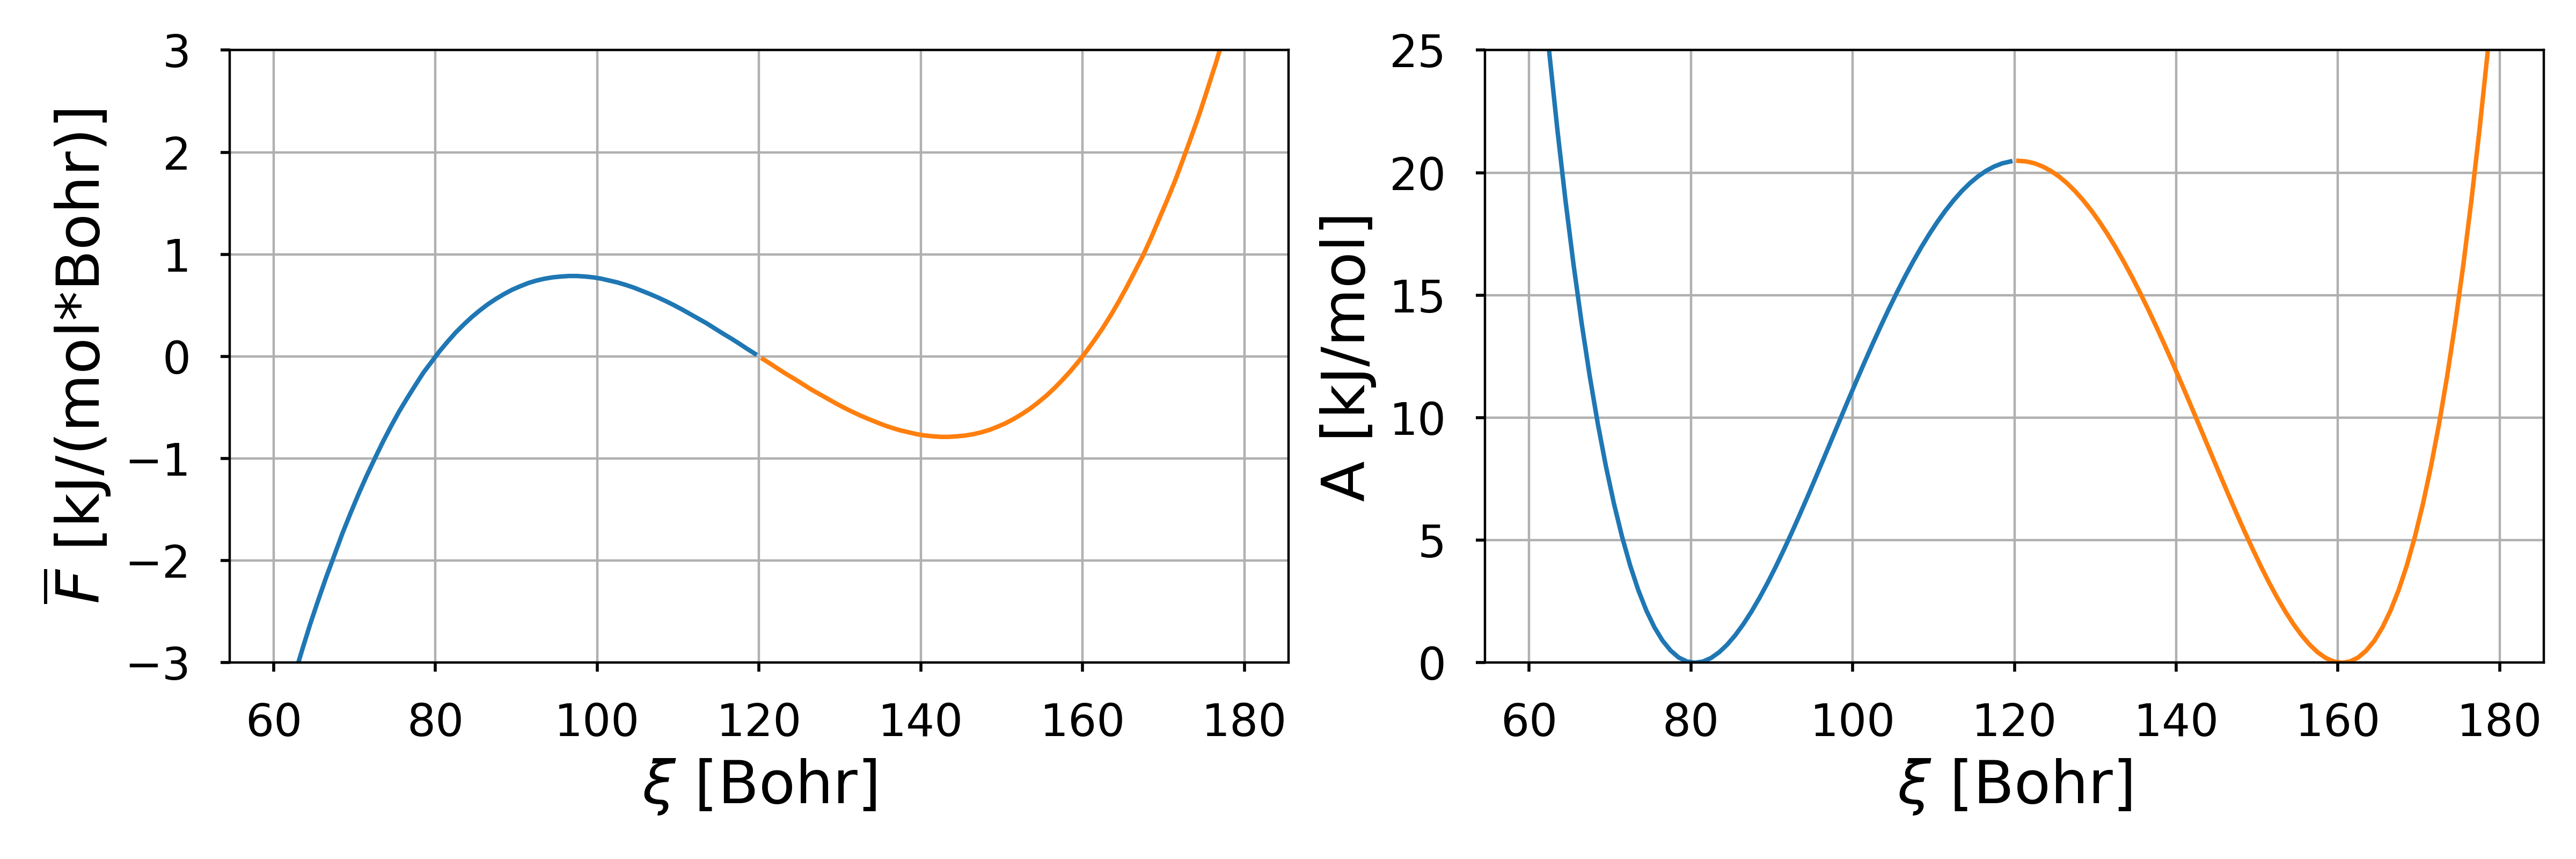
\includegraphics[width=1\textwidth]{bilder/ABF_stratification}
    \caption{Application of the stratification strategy for ABF simulations. $\xi$ is the x-direction. Two simulations are carried out for $\xi=60-120$~Bohr and $\xi=120-180$~Bohr. After both simulations are converged, their force estimates are joined at $\xi=120$~Bohr, as shown on the left.
    Integrating the joined force estimates gives the combined PES shown on the right.
    Details are given in the Appendix.}
\label{fig:stratification}%
\end{figure}

Multiple walker strategies take parallelization one step further by allowing more than one walker to contribute to the same window.
For this purpose multiple schemes were proposed, ranging from simply running similar independent simulations in parallel, to complex ones involving selection rules or replica exchange between simulations at different temperatures.\autocite{wilson2011molecular,comer2014calculation,minoukadeh2010potential}
Here, we will look at a relatively simple scheme, termed \textit{shared adaptive biasing method}\autocite{comer2015adaptive}, where all accumulators $f$ required for the respective method, such as histograms, force estimates, or potentials, are synced between otherwise independent walkers in fixed time intervals. %Global and local accumulators evolve according to the following update scheme
%\begin{enumerate}
%  \item $f_{l}(t_{sync}) \leftarrow f_{g} + \biggl(f_{l}(t_{sync})-f_{l}(t_{sync}-1) \biggr)$
%  \item $f_{g} \leftarrow f_{l}(t_{sync})$
%\end{enumerate}
%where at synchronization times $t_{sync}$ the local accumulators are set to the current global value $f_{g}$ plus the progress of the local walker since the last sync.
For this purpose global contributions $f_g$ are stored in one shared buffer file.
This way all walkers contribute to the same bias and achieve much faster convergence.
Typically the synchronization interval $t_{sync}$ is chosen much bigger than the MD step size.
Most of the time different walkers are located in different bins along the CV and sharing the bias after every MD step would therefore not change the overall dynamics.
This way communication between individual walkers can be kept minimal.
Additionally no master node is needed, as the buffer is simply accessed by each walker in fixed intervals.
To avoid inconsistency, access to the buffer only granted to one walker simultaneously.
If write access to the buffer is denied for a walker, it will share its progress at the next synchronization time.

This scheme, which was developed specifically for ABF simulations, was shown to be particularly useful for complex reactions, for example in biochemical context, where several transition mechanisms can be associated with the same CV and multiple parallel valleys have to be sampled for reliable PMF estimates.\autocite{minoukadeh2010potential}
In this case one walker only visits a small portion of this parallel valleys, as it is trapped in a specific region of configuration-space orthogonal to the CV.
With shared biases every contributing walker can be expected to sample different parallel valleys, which results in more reliable free energy estimates.
